\documentclass[8pt,notitlepage]{report}
\usepackage[utf8]{inputenc}
\usepackage[english]{babel}
\usepackage{amsmath}
\usepackage{amsfonts}
\usepackage{amssymb}
\usepackage{makeidx}
\usepackage{graphicx}
\usepackage{hyperref}
\usepackage{float}
\usepackage{titling}
\usepackage{lipsum}
\usepackage[top=1in, bottom=1.25in, left=1.25in, right=1.25in]{geometry}
\usepackage[justification=justified, format=plain]{caption}
\usepackage[ruled]{algorithm2e}
\usepackage[nameinlink]{cleveref}

\title{PeterPen}
\author{Dario Montagnini, Antonio Musolino, \\Manuel Prandini, Giovanni Varricchione}
\date{}

\graphicspath{ {../images/} }

\begin{document}

\twocolumn
[
	\begin{@twocolumnfalse}
	\maketitle
	\begin{abstract}
		The main goal of this project was the creation of a pen which could be used in handwriting recognition. To this end, we designed a pen with which we can capture data while a person is writing, and then send it to a server through a Wi-Fi connection. The pen has been made with affordable chips and its body with a 3D printer. Two recognition systems have been implemented, one based on deep learning and the other on signal distances. On the available dataset we have observed good performances from both systems, with very interesting findings for the deep learning one. 
	\end{abstract}
  	\end{@twocolumnfalse}
]

\subsection*{Handwriting}
	Handwriting is one of many traits which can be used in a biometric system. It is categorized as a \textit{behavioural} biometric trait, as it is based on an action which the user learns, and also depends on his or her mood, when the data is captured (other examples of this kind of trait are the way one walks and keystrokes). In general, it has a low accuracy but a high acceptability. \\
	The trait mainly depends on the writer's handwriting style, the force applied and the pen's inclination while writing.
\subsection*{State of the art}
	Typical handwriting recognition systems use signature to recognize a user (e.g. Karouni et al. \cite{Karouni15}). In this case we usually talk of "\textit{signature recognition}", and they are mainly based on the assumption that each person has a unique signature and, thus, it can be used as a highly distinctive trait. It is also possible to use general handwriting to recognize a person, in this case instead we refer to "\textit{handwriting recognition}". While the former are vulnerable to \textit{spoofing} attacks, the latter are stronger but can be less accurate. \\ 
	There are two approaches to handwriting recognition: the first, called "\textit{static}" or "\textit{off-line}", uses techniques of \textit{image processing}. The written word (or signature) is captured and then transformed into an image, which afterwards will be analysed by the system (e.g. Sharif et al. \cite{Sharif18} and Souza et al. \cite{Souza18}). The second approach, called "\textit{dynamic}" or "\textit{on-line}", analyses the signals captured by the sensors on the pen. Typical used signals are force, acceleration and rotation, as they can distinguish handwriting. Usually, the latter have better performances than the former ones. \\
	A dynamic approach which is similar to the one which will be presented is the Biopen, by De Marsico M., Ponzi F., Scozzafava F. e Tortora G. \cite{DeMarsico18}. Nonetheless, the two models have some differences. First of all, the Machine Learning system in the PeterPen uses LSTMs, while the BioPen uses SVMs. Moreover, the force which is measured is different: while the BioPen considers the one applied by the user on the pen while holding it, the PeterPen measures the one applied on the tip of the pen while writing. As we measured this kind of force, we were also able to automatize data capturing, considering only the intervals when measured force was higher than a certain threshold. Clearly, these two approaches to the use of force have also influenced user recognition.
	
\chapter{Architecture}
	\begin{figure}[H]
		\begin{center}
			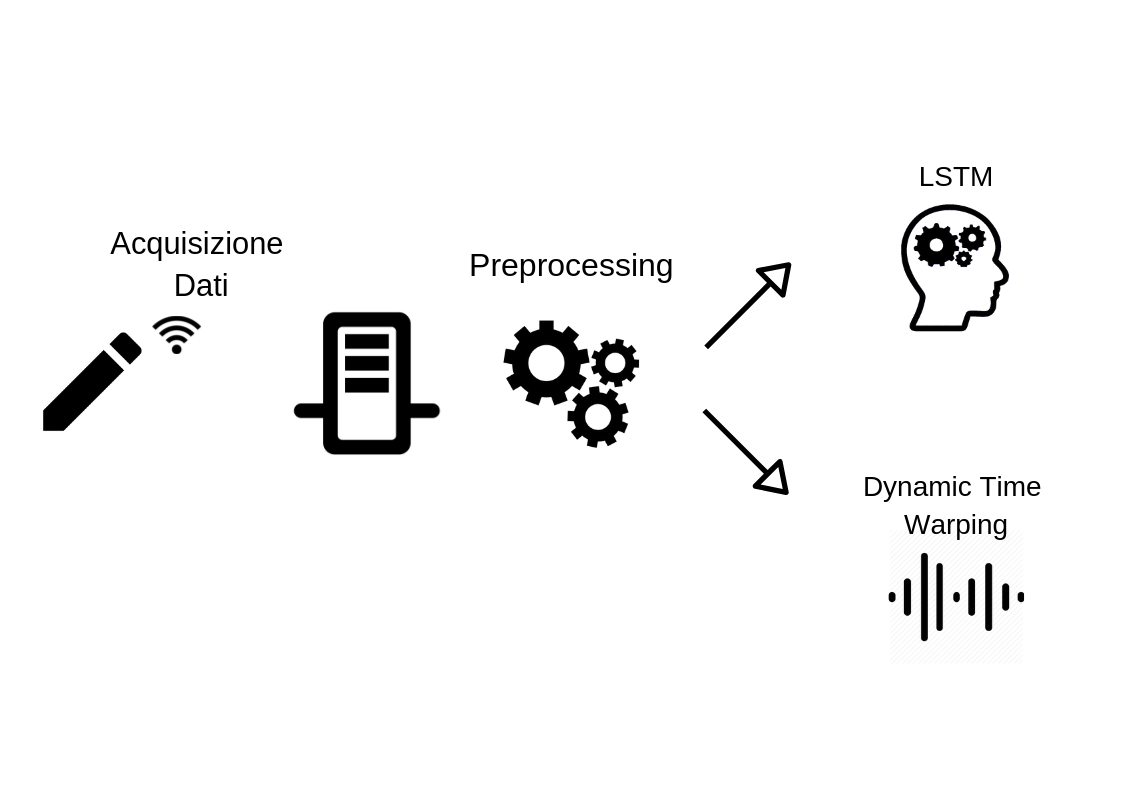
\includegraphics[scale=.25]{architettura}
			\caption{System architecture}
		\end{center}
	\end{figure}		
	The system architecture is made out of 4 elements: the pen, a server which acquires data and the preprocessing and classification modules. The pen gathers data through its sensors and sends them to the server via a Wi-Fi module, which is installed on its chip. JSON files are used to store such data on the server (to each "\textit{writing session}", i.e. the writing of a single word,  a file is associated) and can thus be used by the preprocessing module. This last one has the objective of normalizing data, in order to make them usable by the classifiers. There are two classification modules, the first is a \textbf{Neural Network} which uses  \textbf{LSTMs}, and the second one is based on the \textit{Dynamic Time Warping} algorithm.

	\section{PeterPen}
		The pen is made up of the following hardware:
		\begin{itemize}
			\setlength\itemsep{.1em}
			\item a NODE MCU ESP8266 chip;
			\item an accelerometer;
			\item a gyroscope;
			\item a force sensor;
			\item a green LED;
			\item a capacitor;
			\item two resistors;
			\item a 9V battery;
			\item a PLA case.
		\end{itemize}
		The ESP8266, the main chip, consists of a micro-controller and a Wi-Fi module used to communicate with the server. The accelerometer and the gyroscope (both on a single chip), the force sensor and the LED are connected to this chip. \\
		The sensor is able to measure the force applied on the pen tip thanks to a spring. Right after the force sensor there is the accelerometer and gyroscope chip and, after this, the ESP8266. \\
		
		\begin{figure}[H]
			\begin{center}
				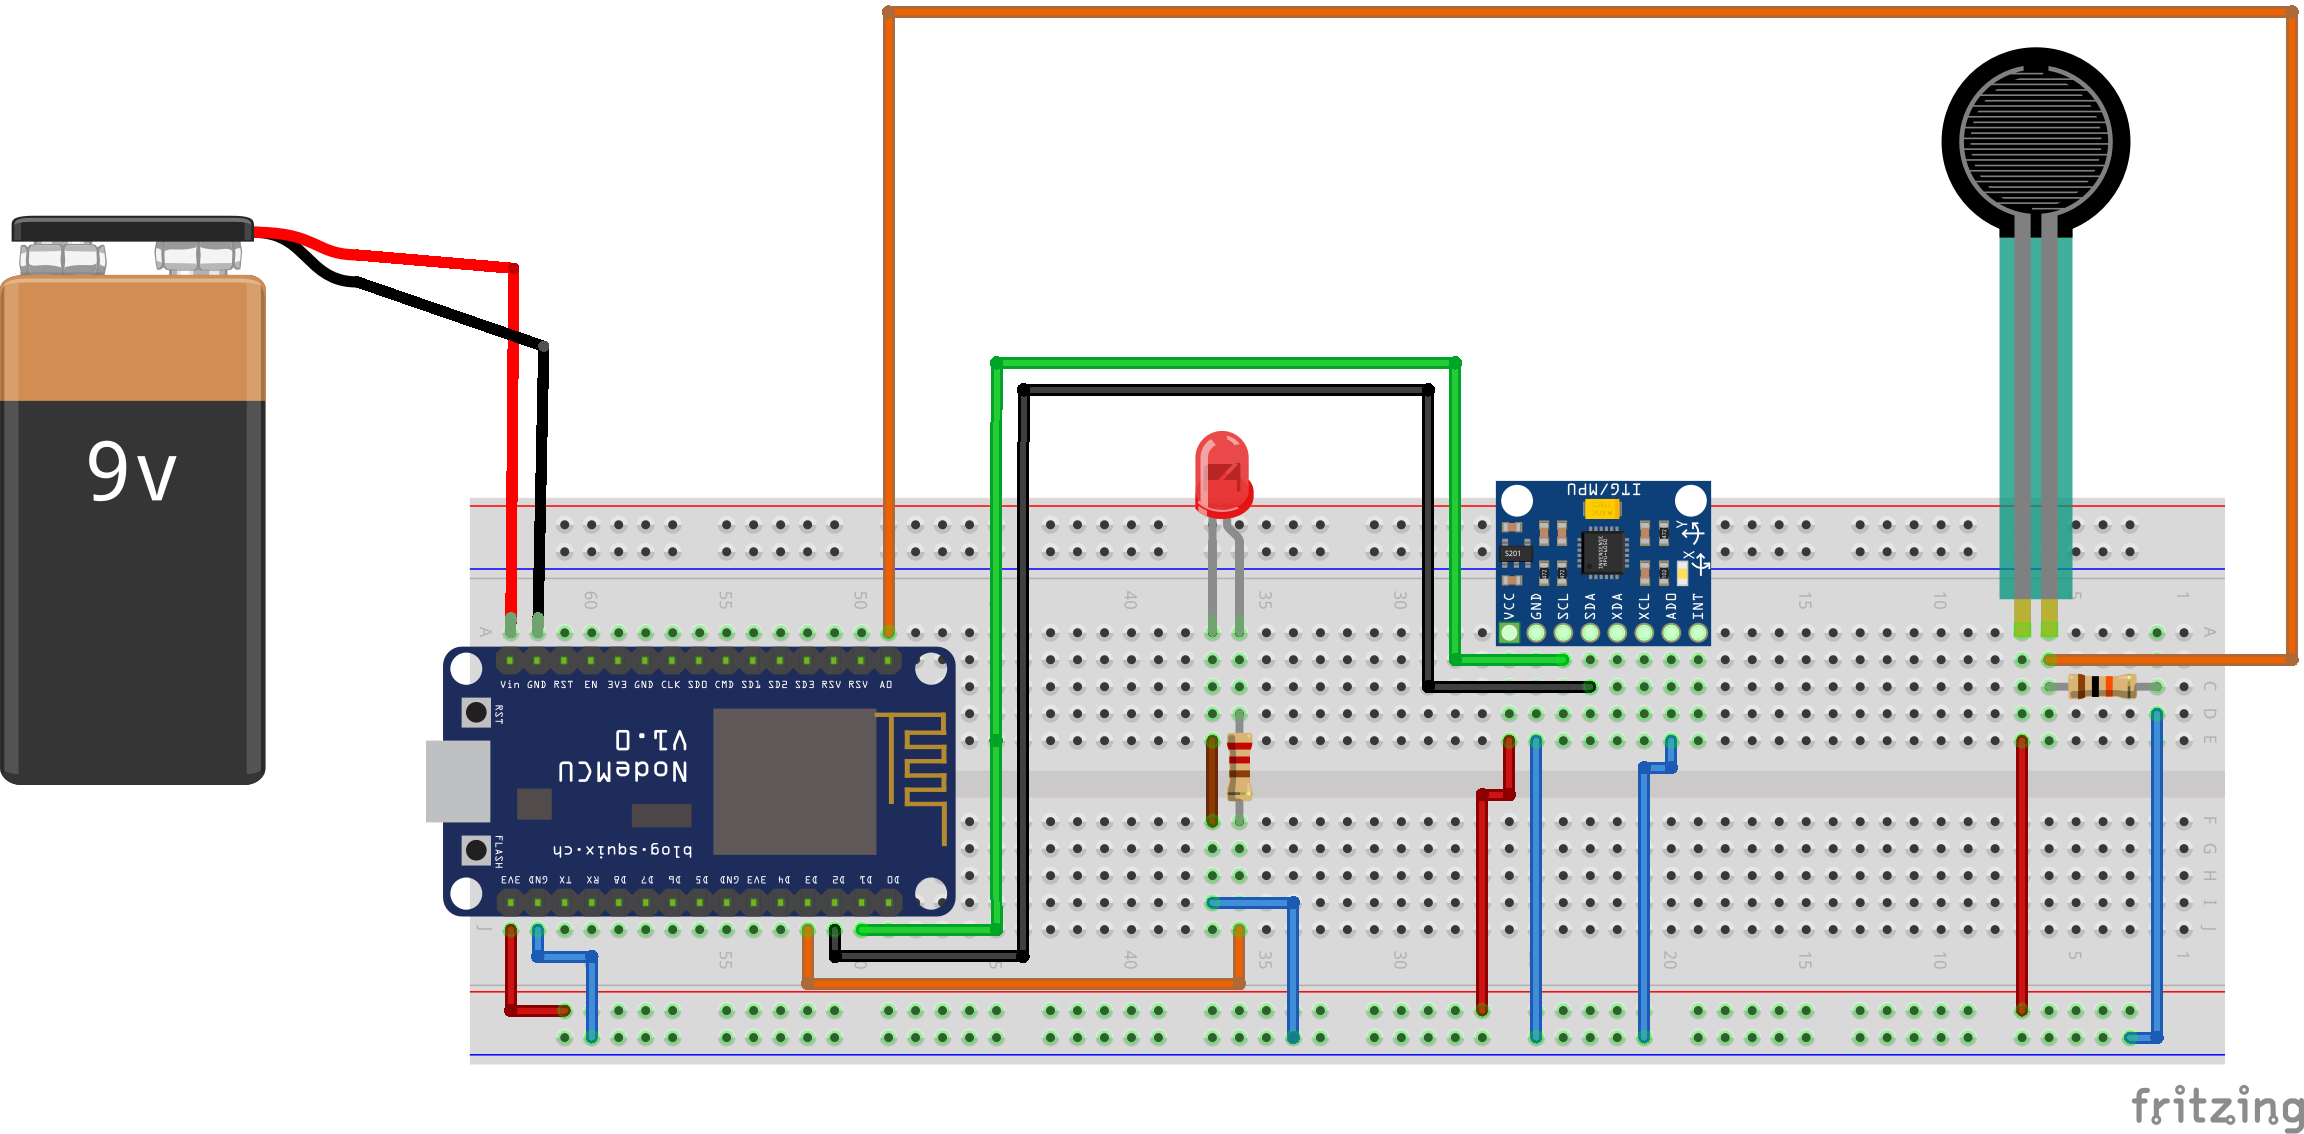
\includegraphics[scale=.35]{circuito}
				\caption{PeterPen electrical network}
				\label{fig:circuito}
			\end{center}
		\end{figure}

		\begin{figure}[H]
			\begin{center}
				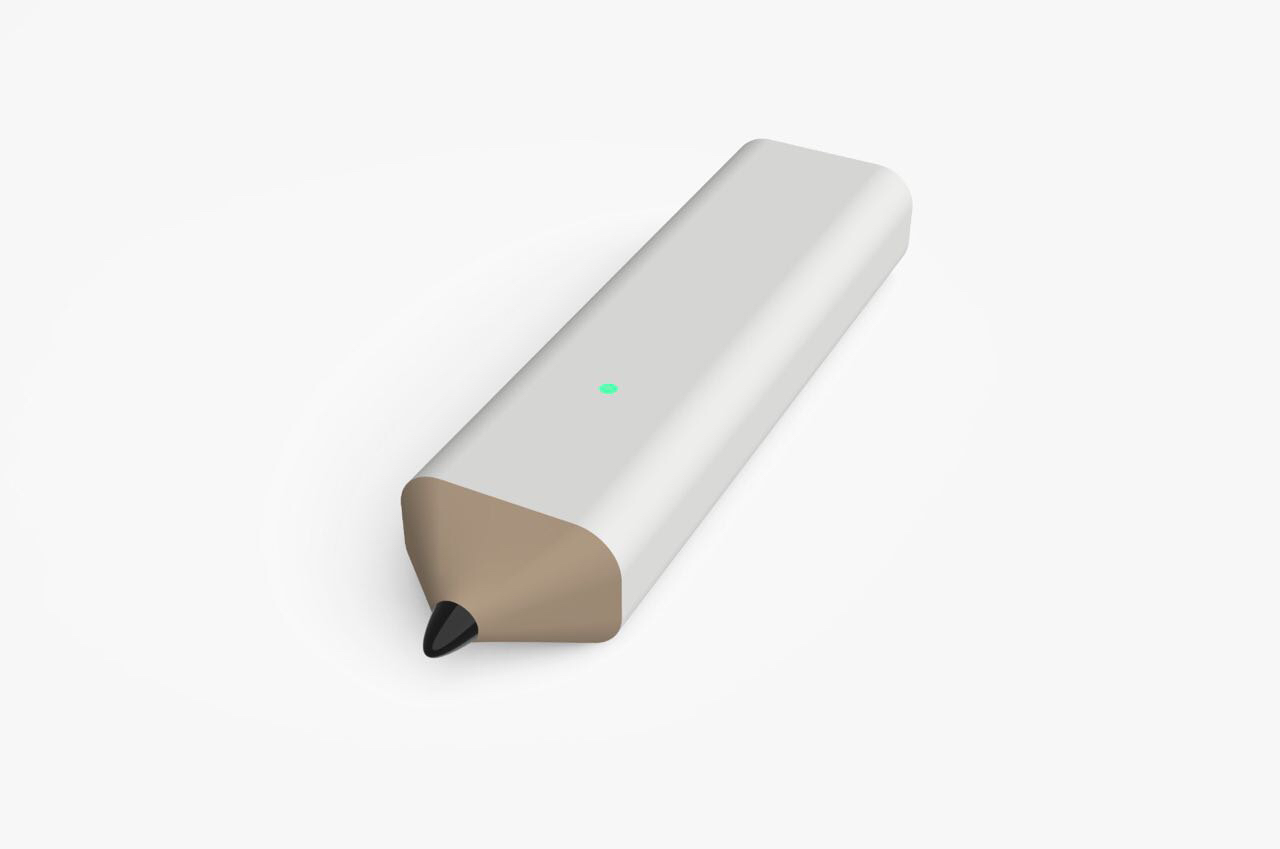
\includegraphics[scale=.1]{design}
				\caption{PeterPen design, we would like to thank Cristian Cianfarani and Tiziano Grossi}
			\end{center}
		\end{figure}		
		
		\begin{figure}[H]
			\begin{center}
				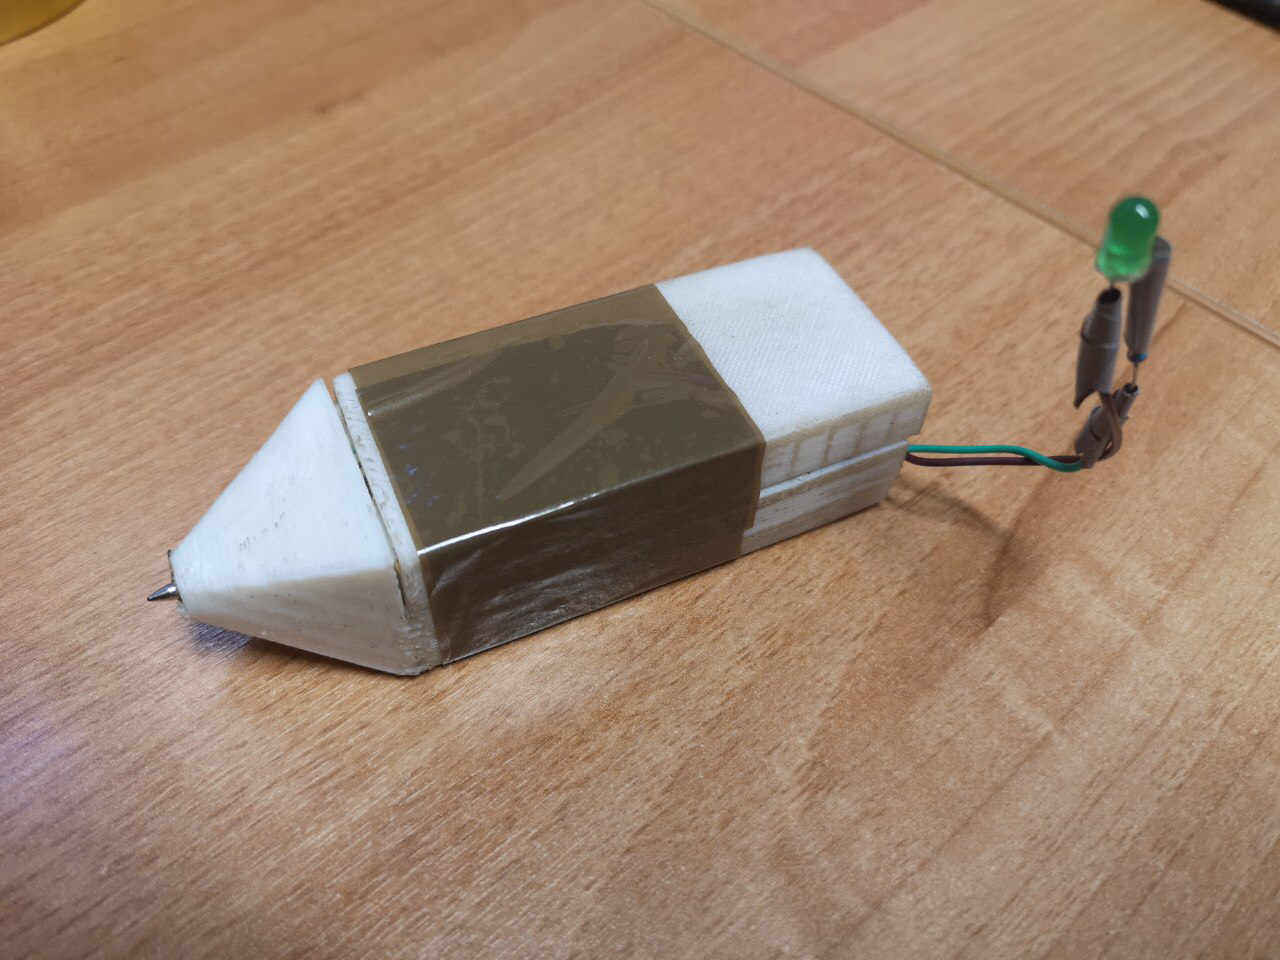
\includegraphics[scale=.105]{peterpen}
				\caption{PeterPen}
			\end{center}
		\end{figure}
		

		\subsection{Acquisition protocol}
			We designed an acquisition protocol to simplify the data capture process. The pen can be powered up through a USB cable or a battery, using a 9V one (\cref{fig:circuito}) or a 3.3V or 3.6V one (using the 3v3 pen for the latter ones); when it is turned on, the LED blinks while trying to connect to the network and the server, otherwise, it blinks if there is an error. Once connected, the LED stops blinking and remains on, this signals to the user that he can start writing. While writing the light is turned off and, if no force is detected for more than 2 seconds, it turns on once again, signalling the end of the writing session and the sending of data to the server. Each writing session can last up to a maximum of 10 seconds, if the user exceed such threshold then the LED will blink to signal the error, and no data will be sent.
		
		\subsection{Pen source code}
			The ESP8266 micro-controller has been programmed using the same language to program Arduino chips, which is a C derivative. This particular language requires the implementation of two functions in each program. \\
			The first one, \verb|void setup()|, is executed once at the beginning and initializes variables. The second one, \verb|void loop()|, is the program's kernel and is repeatedly executed as long as the chip is turned on, in our case every 10 milliseconds. \\
			In the \verb|void setup()| function we have implemented, two other functions are called: \\ \verb|mpu6050Begin|, which initializes the accelerometer and gyroscope chip, and \verb|connect|, which connects the chip to the server. The function \verb|loop| at each iteration reads the force sensor value and, based on the state (which is one between \verb|READY|, \verb|WRITING| and \verb|ERROR|) and the variable \\ \verb|counter_writing| will behave differently. \\ If the measured force is enough and the state is \verb|READY|, then the pen moves to the state \verb|WRITING|, gathers data and initializes the counter \\ \verb|counter_writing|. If the force is above a certain threshold, the state is \verb|WRITING| and less than 10 seconds have passed since the user started writing, then data are acquired; otherwise, if 10 or more seconds have passed, the pen moves to the \verb|ERROR| state. Finally, if the state is \verb|WRITING| and at least 2 seconds have passed since not enough force is measured, data is sent to the server and the pen moves to the state \verb|READY|.
			
	\section{Server}
		The server has been programmed with Node.js, open on port 8080 via a TCP socket. At each new connection a new JSON file is created in which the server will store all data received by the PeterPen, after parsing them. When the connection is closed, the server closes its file. 
		
		\subsection{JSON file}
			The file contains a word array, and each word comprises of a length-variable sequence (but long at most 1000) of arrays, each of which contains all the 7 features. \\
			The features are the following:
			\begin{enumerate}
				\setlength\itemsep{.1em}
				\item $ x, y $ and $ z $ accelerometer components;
				\item force value;
				\item $ x, y $ and $ z $ gyroscope components.
			\end{enumerate}


\chapter{Classification}

	\section{Preprocessing}
		In the preprocessing phase data have been normalized, rescaling every feature, and padding has been added to make arrays long exactly 1000. Padding has been added for both models, while rescaling has only been done for the DTW module; as it worsened the NN performance, we decided to keep the data raw for that module. \\ 
		
		\subsection{Normalization}
			Data have been normalized using the following rescaling function: 
			\[ rescaling(x) = \frac{x - min}{max - min} \]
			To this end, we used the following maximum and minimum values:
			\begin{itemize}
				\setlength\itemsep{.01em}
				\item $ \pm 250 $ for accelerometer data;
				\item $ 0 $ and $ 1024 $ for force data;
				\item $ \pm 2 $ for gyroscope data.
			\end{itemize}
	
	\section{DTW}
		DTW (\textit{Dynamic Time Warping}) is a dynamic programming algorithm which measures the similarity of two time sequences; the algorithm is also capable of recognizing sequences which vary in length. In our case, a trivial example is given by a user who, when writing the same word, takes less time in writing it in the first time than in the second. \\
		DTW finds the \textit{optimal matching} between two sequences with the following restrictions and rules:
		\begin{enumerate}
			\item each element of a sequence must be associated at least to another of the other one (but not necessarily just one);
			\item the first element of the first sequence must be associated to the first of the second one;
			\item the last element of the first sequence must be associated to the last of the second one;
			\item matching must be \textbf{monotonous} and \textbf{crescent}, i.e. given two indexes of the first sequence $ i, j $, s.t. $ i < $, then there cannot exist two indexes of the second sequence $ k, q $, s.t. $ k < q $ and $ q $ has been associated to $ i $ and $ k $ to $ j $.
		\end{enumerate}
		To each \textit{matching} a cost is associated, usually the sum of the euclidean distances between associated indexes (which we used in out implementation), and the optimal one is the one with the least cost. 
		\begin{algorithm}[h]
			\SetAlgoLined
			\caption{DTW}
			\KwData{$ s_1: [1 \dots n], s_2: [1 \dots m] $}
			\KwResult{least distance between the two sequences}
				$ \text{DTW } :=  [0 \dots n, 0 \dots m] $ \\
				\For{i := 0 to n }{
					$ \text{DTW}[i, 0] $ := $ \infty $
				}
				\For{j := 0 to m }{
					$ \text{DTW}[0, j] $ := $ \infty $
				}
				$ \text{DTW}[0, 0] = 0 $ \\
				\For{i := 1 to n}{
					\For{j := 1 to m}{
						$ \text{cost } := d(s_1[i], s_2[j]) $ \\
						$ \text{DTW}[i, j] = \text{cost } + $ \\ $  \min(\text{DTW}[i - 1, j], $ \\ $ \text{DTW}[i, j - 1], \text{DTW}[i - 1, j - 1]) $						
					}
				}
				$ \textit{return } \text{DTW}[n, m] $
		\end{algorithm}
		
		The algorithm creates a $ n \times m $ matrix, where $ n $ and $ m $ are, respectively, the two sequences' length, and fills each matrix cell $ i, j $ with the least cost to reach it from the cell $ [0, 0] $; output is thus given by the value in cell $ [n, m] $. The algorithm has a complexity of $ O(nm) $.\\
		We have implemented the algorithm in two versions; for the first, which executes the pseudo-code written above, we have used a GitHub library, which can be found at the following link: \href{https://github.com/pierre-rouanet/dtw}{github.com/pierre-rouanet/dtw}. Instead, the second one consists of an approximation of the algorithm, with a quicker execution but which can, of course, incur in some performance issues; we have used the GitHub library which can be found at the following link: \href{https://github.com/rtavenar/cydtw}{github.com/rtavenar/cydtw}. We will refer to this version of DTW in the rest of the report with the name \textit{Fast}-DTW (FDTW).

	\section{LSTM}
		LSTMs (\textit{Long Short Term Memory}) are a RNN (\textit{Recurrent Neural Network}) architecture. RNNs are a NN family in which output of a given instant $ t $ acts also as input to the network in the following instant $ t + 1 $. One of the internal layers is used a memory, and this lets the network recognize sequences of values, using both the input at time $ t + 1 $ and the internal state (which has been obtained from the input sequence up to instant $ t - 1$).
		
		\begin{figure}[H]
			\begin{center}
				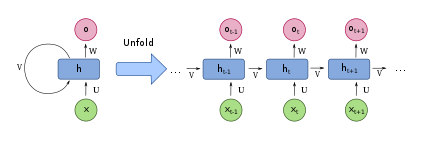
\includegraphics[scale=.55]{rnn}
				\caption{An "unwrapped" RNN}
			\end{center}
		\end{figure}

		A big issue with RNN is that, using \textit{back-propagation} to upgrade its weights, the gradients can vanish (and reach $ 0 $) or explode. In the first case, we can imagine that the RNN forgets information seen "too much time ago". \\
		To solve this, LSTMs can let the gradient flow through without modifying it when it is used as input for the next instant. In detail, the network uses a layer to decide how much "remember" a certain information, multiplying its value by a number between $ 0 $ and $ 1 $ (note the multiplication in the upper left-hand corner in the cell). 
		
		\begin{figure}[H]
			\begin{center}
				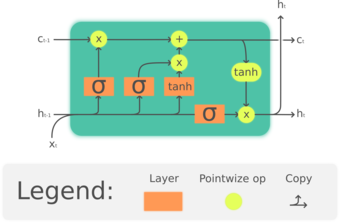
\includegraphics[scale=2.2]{lstm}
				\caption{LSTM architecture}
			\end{center}
		\end{figure}		
		
		As we can observe from the picture, an LSTM cell comprises of many layers, 3 which use sigmoid as their activation function and 1 with hyperbolic tangent activation.
		In detail:
		\begin{itemize}
			\item the layer to the far left is called "\textit{forget gate}", and its output modifies the previous gradient;
			\item the two central layers are called "\textit{input gate}", the sigmoid-activated one decides which information will be added to the network's memory, while the hyperbolic tangent-activated one outputs the new values which could be added. The following \textit{point-wise} multiplication gives the array of values which are to be added to the memory;
			\item the layer to the far right is called "\textit{output gate}", and modifies the network's final output.
		\end{itemize}
		
		\subsection{Model architecture}
			The implemented \textit{deep learning} model is made up of 5 layers, of which 2 are LSTMs (\cref{fig:model}):
			\begin{enumerate}
				\item a first \verb|Masking| layer;
				\item two \verb|LSTM| layers;
				\item a \verb|Dropout| layer;
				\item a finale \verb|Dense| layer.
			\end{enumerate}
			
				\subsubsection{Masking}
					The \verb|Masking| layer is used to remove padding, which makes learning cheaper. It should be observed that we used padding for the deep learning model as well because in this way, we can give any sequence to it in input, overcoming the issue of the variable length (which instead will always be 1000 thanks to padding).
					
				\subsubsection{LSTM}
					The two \verb|LSTM| layers are consecutives, the first has the option \verb|return_sequences| activated, in order to pass the whole sequence of arrays in input to the next layer, and not just the last one. Initially we used only one \verb|LSTM| layers, however we have observed that this two-layer version offers better performances; moreover, adding a second layer allowed us to have a layer which gave in output the whole processed sequence, which could furtherly be analysed by the other \verb|LSTM| layer.
					
				\subsubsection{Dropout}
					The \verb|Dropout| layer changes some random inputs to $ 0 $, to try to prevent \textit{overfitting}. Such probability in the implemented model is $ 0.5 $.
					
				\subsubsection{Dense}
					The \verb|Dense| layer outputs the classification, using the sigmoid as its activation function.					
			
	
			\begin{figure*}
				\begin{center}
					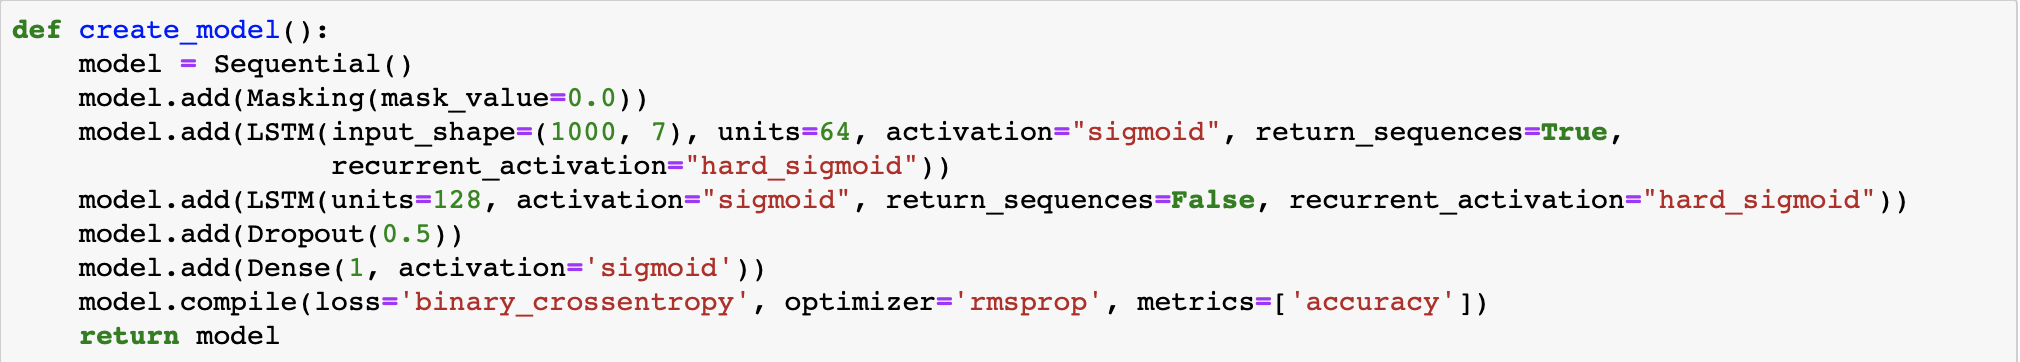
\includegraphics[scale=.45]{def_model}
					\caption{Model definition}
					\label{fig:model}
				\end{center}
			\end{figure*}					
					
			\begin{figure*}
				\begin{center}
					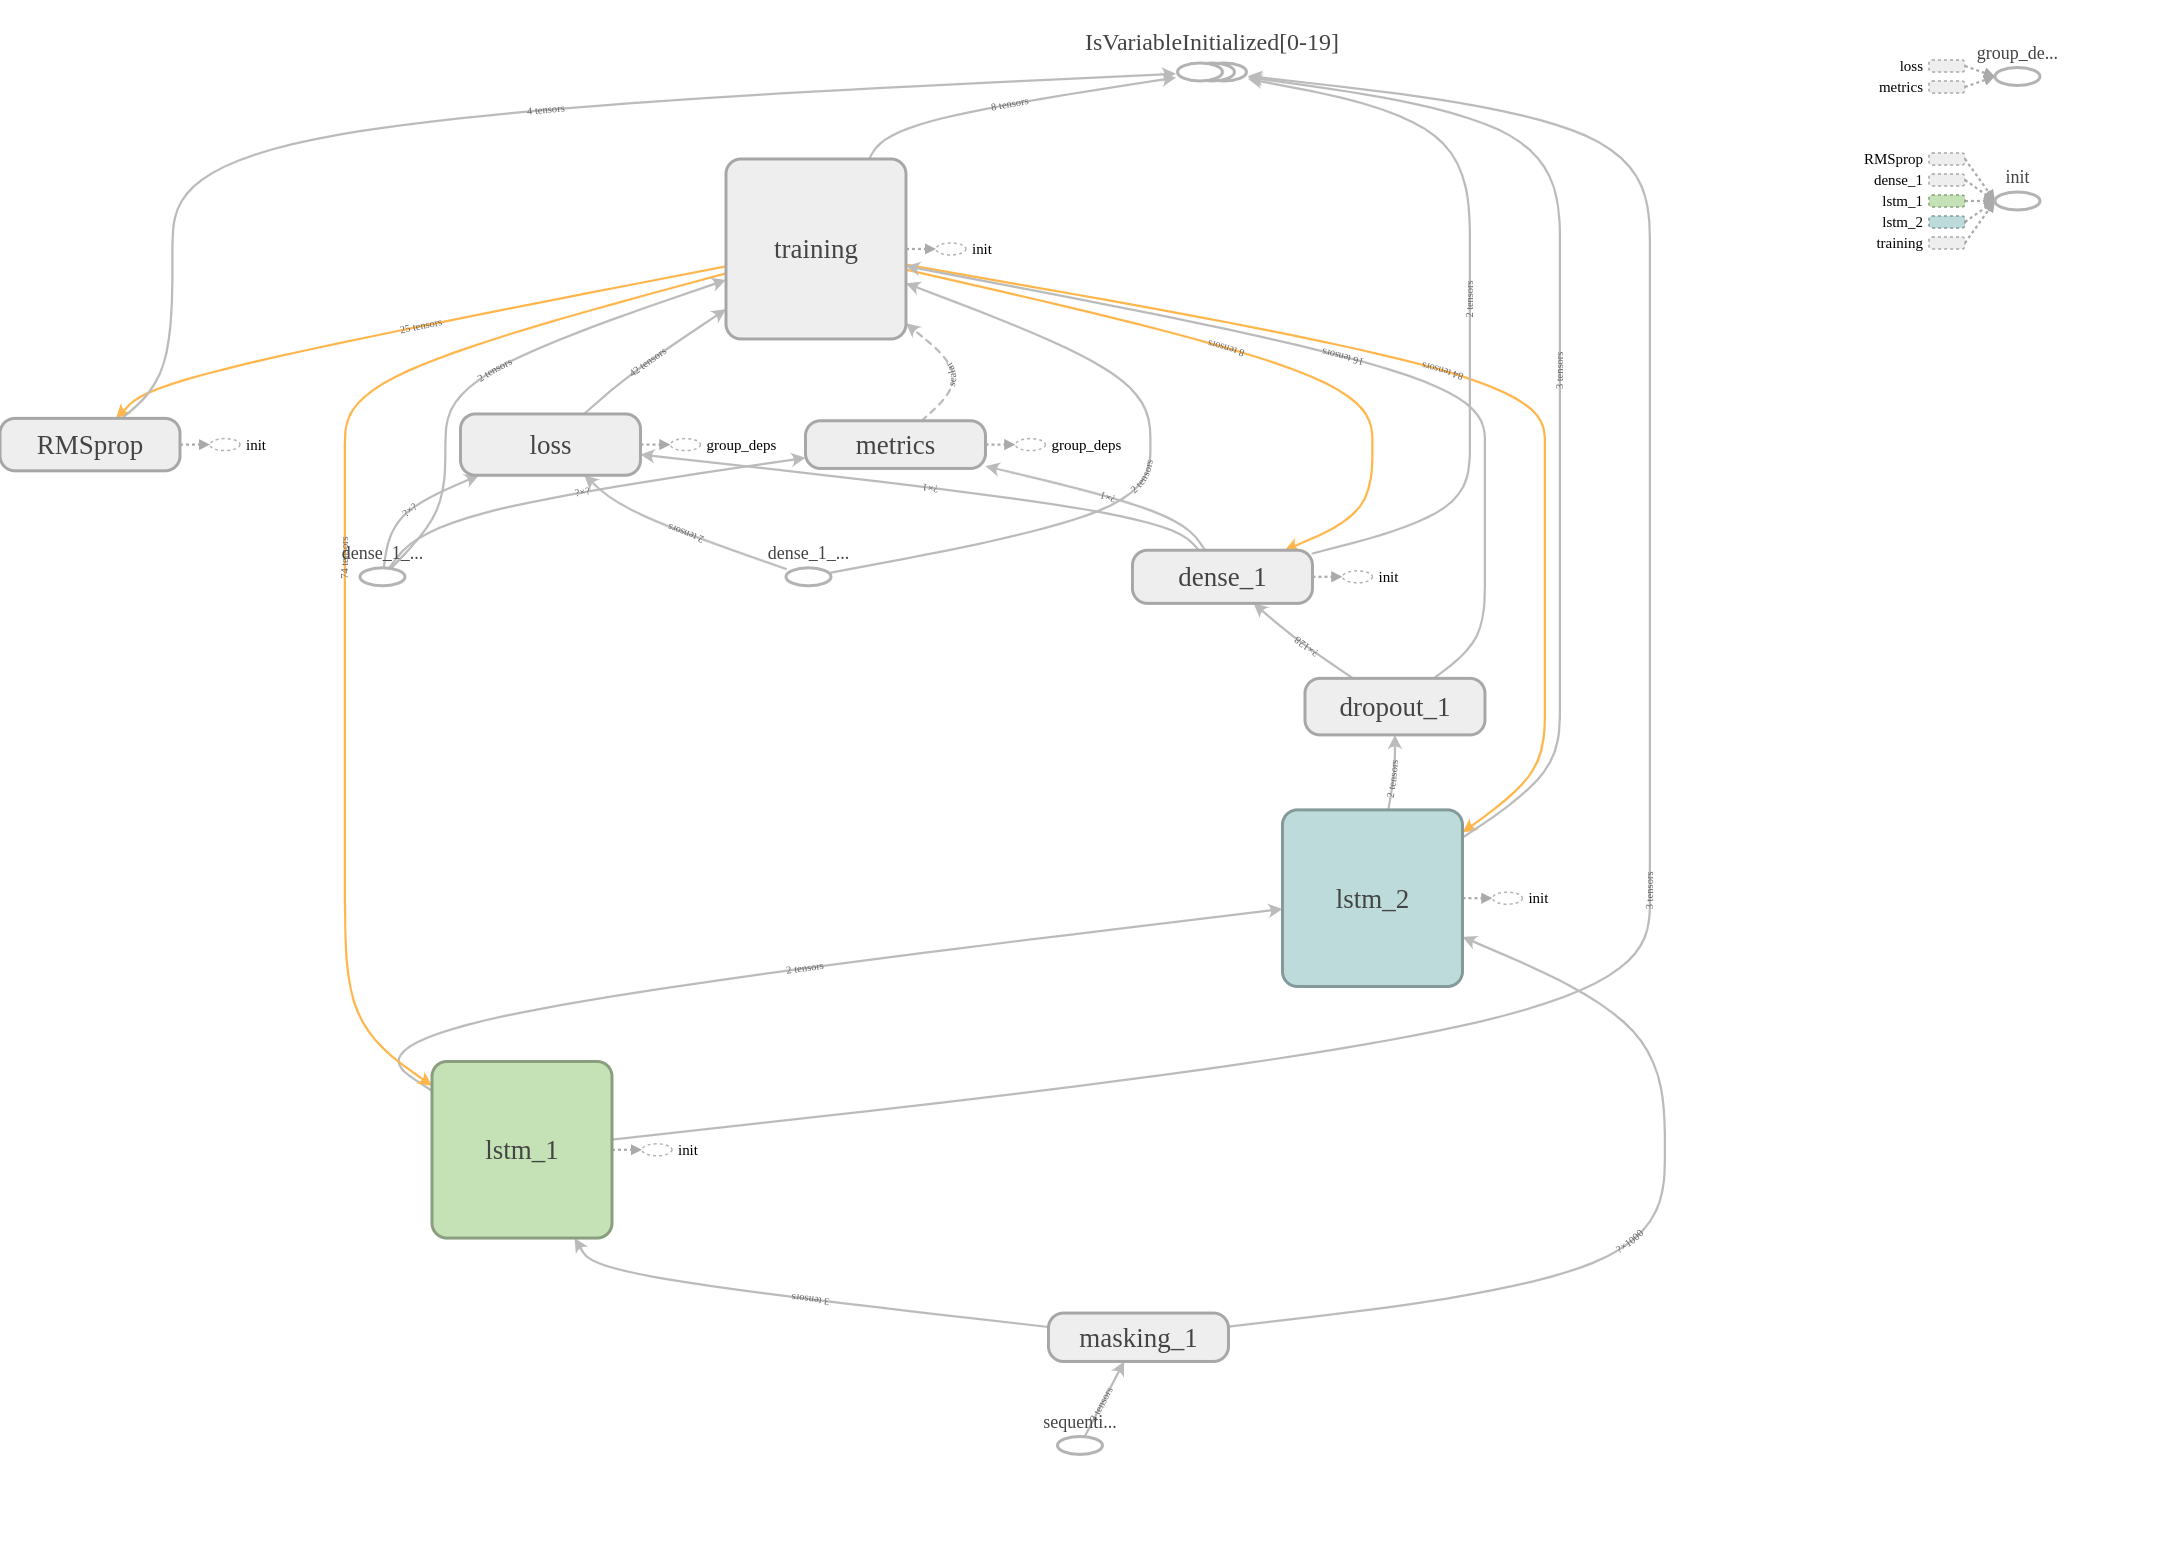
\includegraphics[scale=.23]{lstm_model}
					\caption{Model during training phase, represented by TensorFlow}
				\end{center}
			\end{figure*}		
		


\chapter{Training and testing}
	The collected dataset contains the words written by 23 different users, counting up to a total of 845 samples. The chosen word was "Computer", written in italics. \\
	Both training and testing have been executed on the following machine:
	\begin{itemize}
		\item CPU: Intel Core i7 8700K;
		\item GPU: NVIDIA GeForce GTX 1070;
		\item RAM: 32 GB @ 3200 MHz.
	\end{itemize}
	
	\subsubsection*{Docker}
		In order to exploit the GPU's power we have used Docker. Docker is a virtualization system which creates virtual machines, called "\textit{containers}", who share a common kernel (thus allowing for better performances when compared to a simple virtual machine). We have implemented a container in which a Jupyter Notebook is executed. The system has also facilitated deploy, making it possible from every machine (since Jupyter Notebooks can be executed from remote) and providing higher protection against security attacks (as the program is executed inside a virtual machine). 
	
	\section{Training}
		The deep learning system has been trained on different users, giving a different model for each one of them. \\
		Each training lasted 110 epochs, with batches of 32 elements; moreover, in each epoch a validation phase has been done, using a third of the words in the training set. \\
		Clearly, the available dataset is still rather small, hence the results which will be given in the following section are not truly indicative of the system's real performances. However, an analysis to have some first impressions is important as well.
		
	\section{Testing}
		
		\subsection{DTW}
			Concering DTW we, unfortunately, we able to perform a limited number of tests, especially due to time issues. Since Python does not support multithread execution, the program has been executed on a single core, making it slower. \\
			Nonetheless, promising results have been obtained:
				\begin{figure}[H]
					\begin{center}
						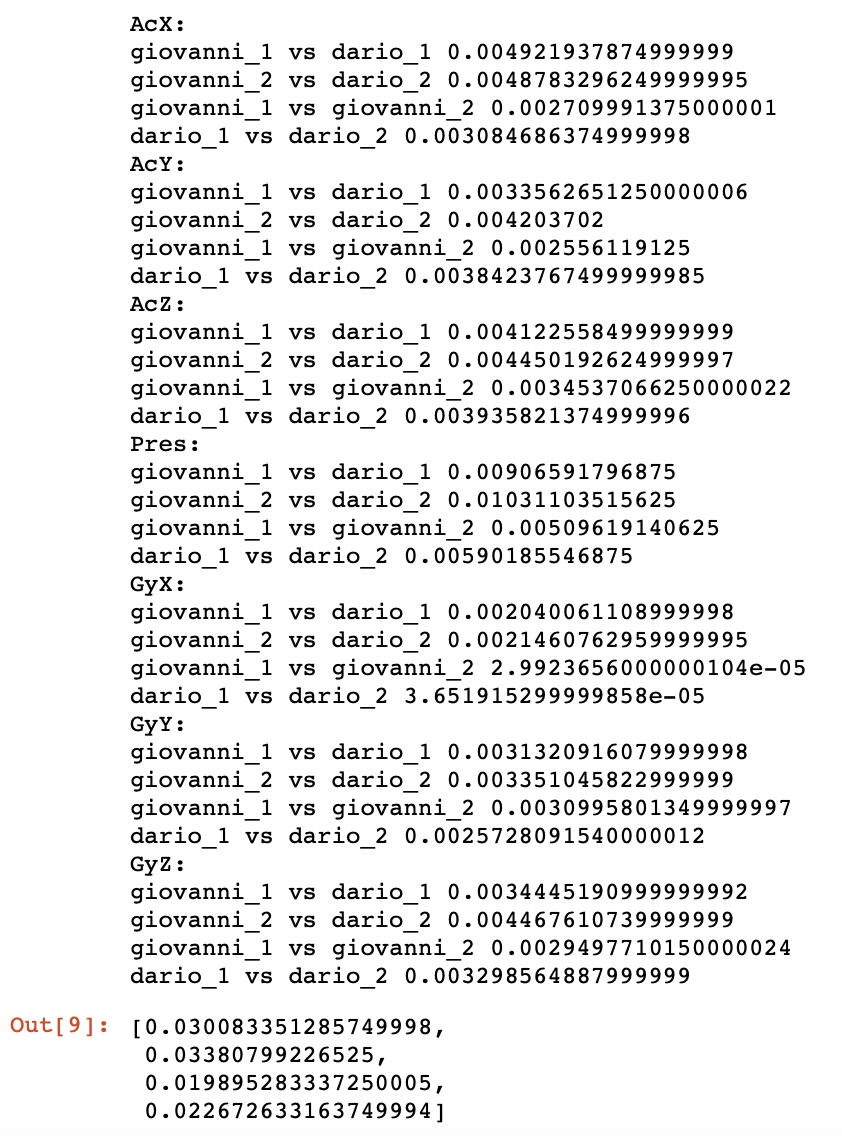
\includegraphics[scale=.25]{dtw_test}
						\caption{DTW results on two pairs of words from two registered users}
					\end{center}
				\end{figure}	
				
			For each DTW test (this is only one of those we have performed) we consider a pair of words per user and compare them to another pair of words from another user. For each component (accelerometer, force, gyroscope) we output the distances for each combination between the four words; finally, we print an array which contain the sum of the relative distances for each one of the words pairs.  \\
			Ideally, pairs from two different users should have an overall distance greater than the one of a couple from the same user. What we have been able to observe, with the few tests we have done, is that this assumption is true in all the cases. \\
			In a second kind of test, which we have tried only once as it took approximately between 6 and 7 hours, we have randomly selected a word from the dataset and evaluated its distance (as the average of all the 7 components) from the rest of the available words. The test has been very positive, giving a ROC curve with an AUC very close to $ 1 $:
			
			\begin{figure}[H]
				\begin{center}
					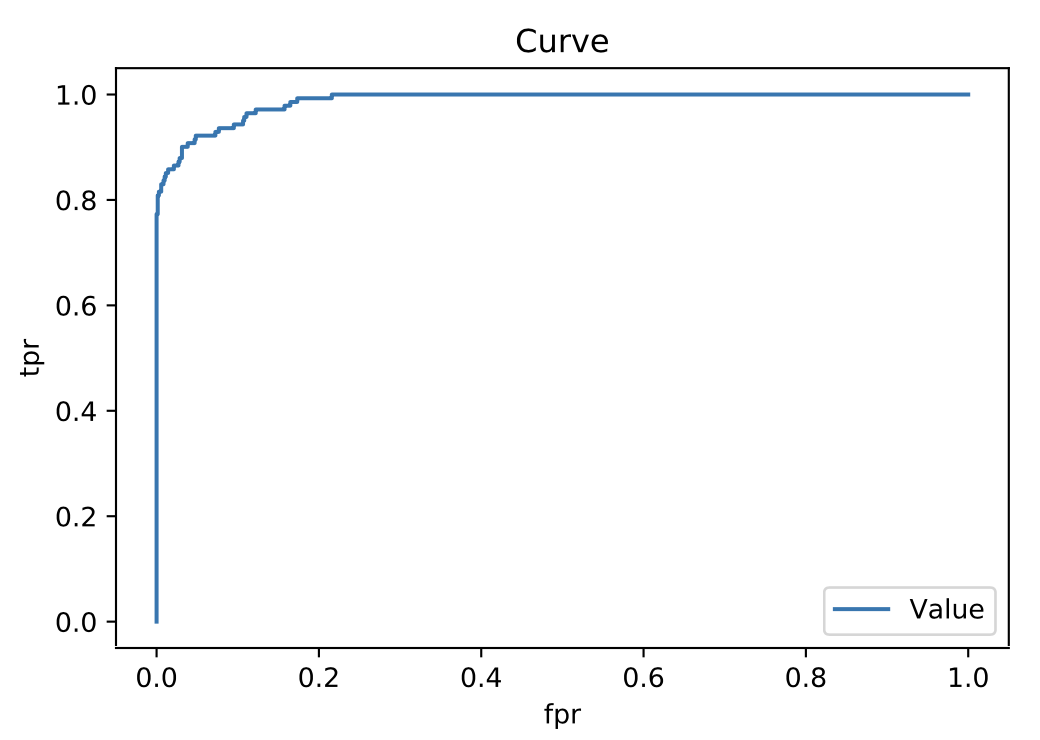
\includegraphics[scale=.4]{ROC_DTW_Antonio}
					\caption{ROC curve obtained considering "vicinity" ($ 1 - d $); AUC $ \cong 0.99 $}
				\end{center}
			\end{figure}
			
			Since features have been scaled between $ 0 $ and $ 1 $, the max distance is exactly $ 1 $, hence vicinity is the difference between $ 1 $ and the evaluated distance.
			
			\begin{figure}[H]
				\begin{center}
					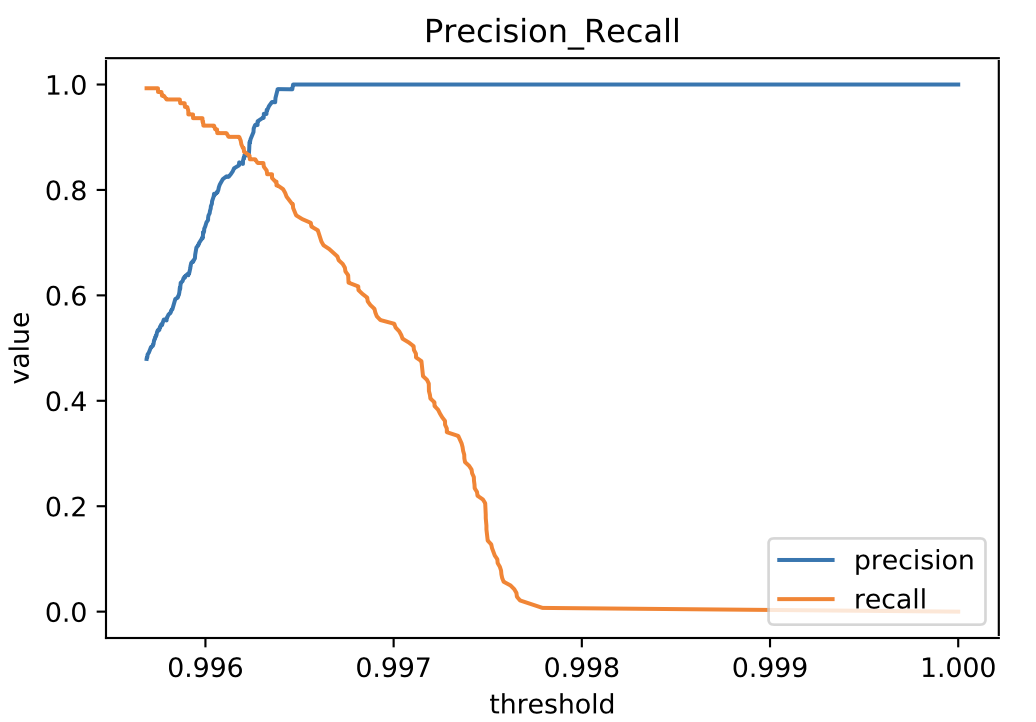
\includegraphics[scale=.45]{precision_recall_DTW_Antonio}
					\caption{Precision and recall curves as the threshold changes}
				\end{center}
			\end{figure}
			
			\begin{figure}[H]
				\begin{center}
					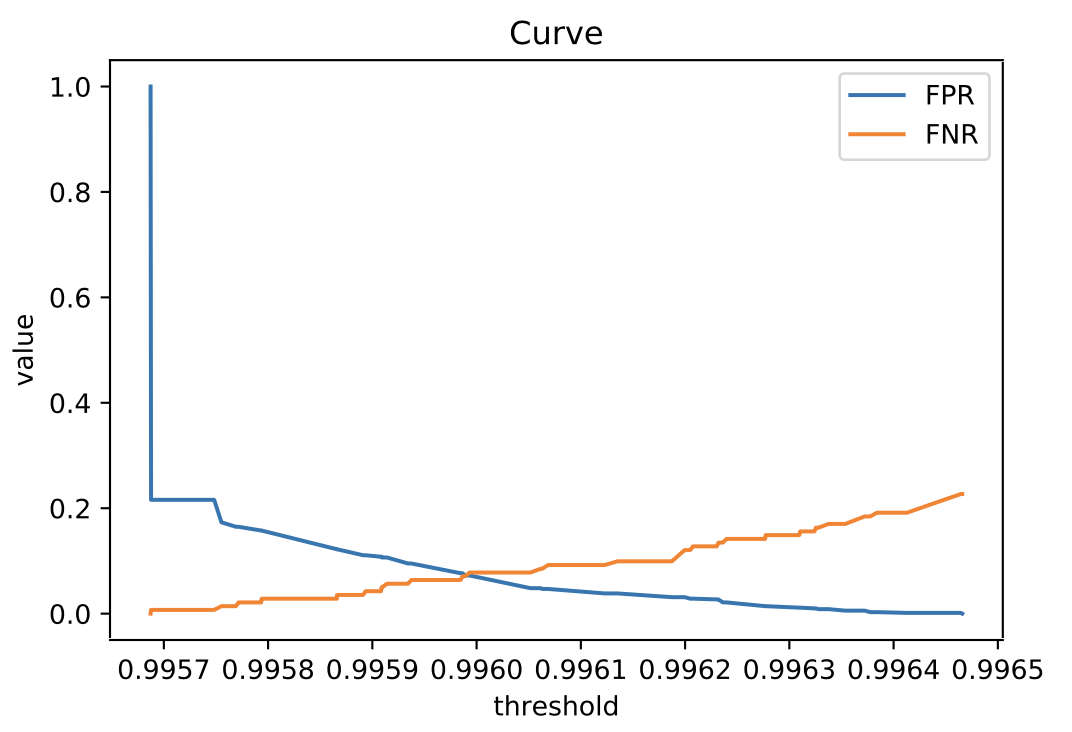
\includegraphics[scale=.45]{fpr_fnr_DTW_Antonio}
					\caption{FPR and FNR curves as the threshold changes, observe how EER is less than $ 0.1 $, with the relative threshold just belo $ 0.996 $}
				\end{center}
			\end{figure}
		
		\newpage		
		
		\subsubsection{FDTW}
			With \textit{Fast}-DTW we were able to perform many more tests. \\
			Our hypothesis that it would have worse performances compared to DTW has been confirmed, however we have observed that data quality (i.e. how much noise was in data) has heavily weighed on this. To sum it up, FDTW highlights DTW issues, that is, that it can't "correct" wrong data. If a user writes in a very different way the same word, these algorithms which analyze signals will clearly have worse performances, whereas a deep learning model could, in some way, understand that the user is the same, even if data are much different. For "vicinity" between two words $ s_1, s_2 $ we used the ratio $ \frac{1}{1 + d(s_1, s_2)} $ in these tests. 
			
			\begin{figure}[H]
				\begin{center}
					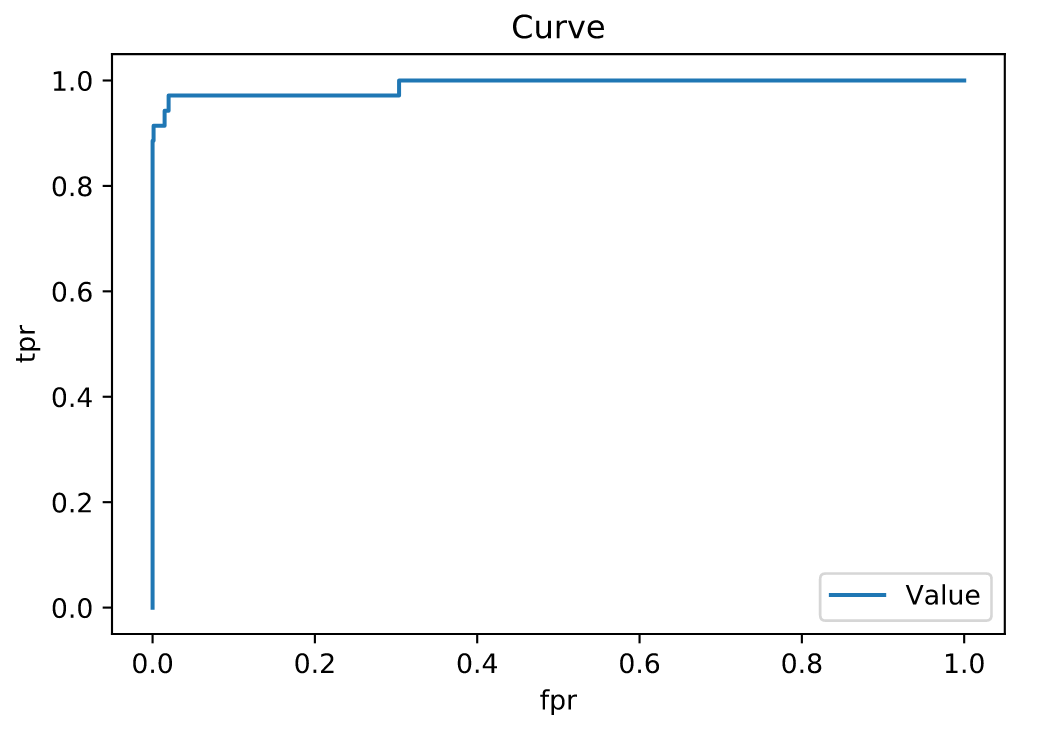
\includegraphics[scale=.35]{ROC_FDTW_Giovanni}
					\caption{ROC curve of one of the best FDTW performances;\\ AUC $ \cong 0.99 $}
				\end{center}
			\end{figure}
			
			\begin{figure}[H]
				\begin{center}
					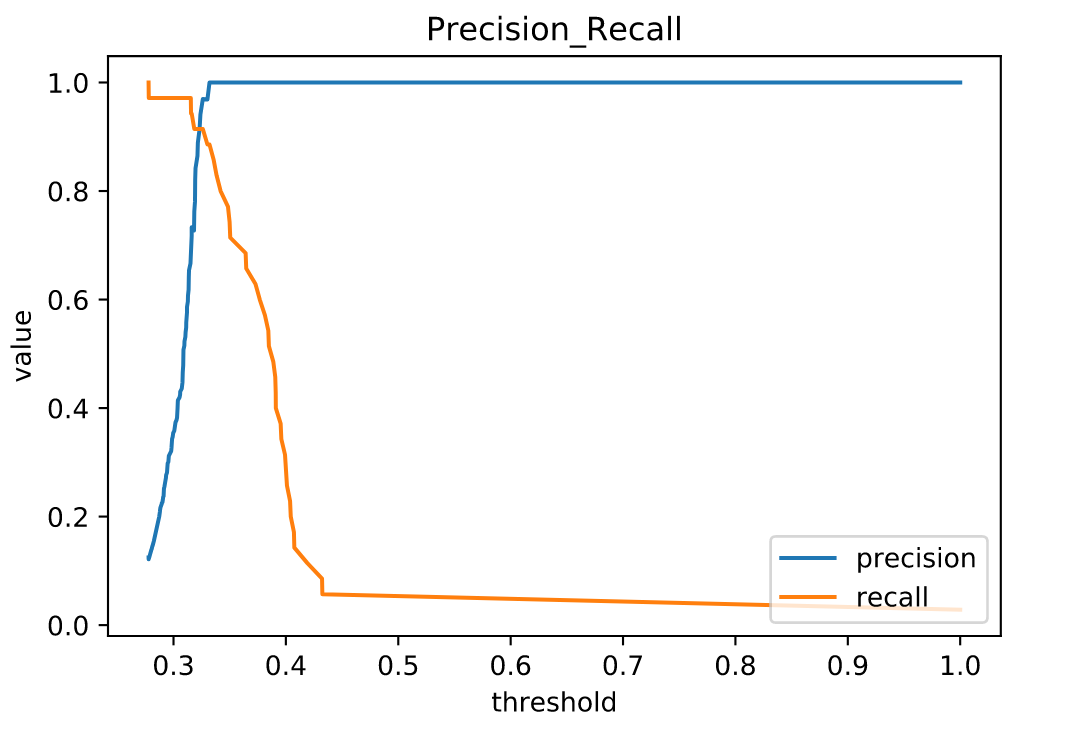
\includegraphics[scale=.35]{precision_recall_FDTW_Giovanni}
					\caption{Precision and recall curves for the same user}
				\end{center}
			\end{figure}
			
			\begin{figure}[H]
				\begin{center}
					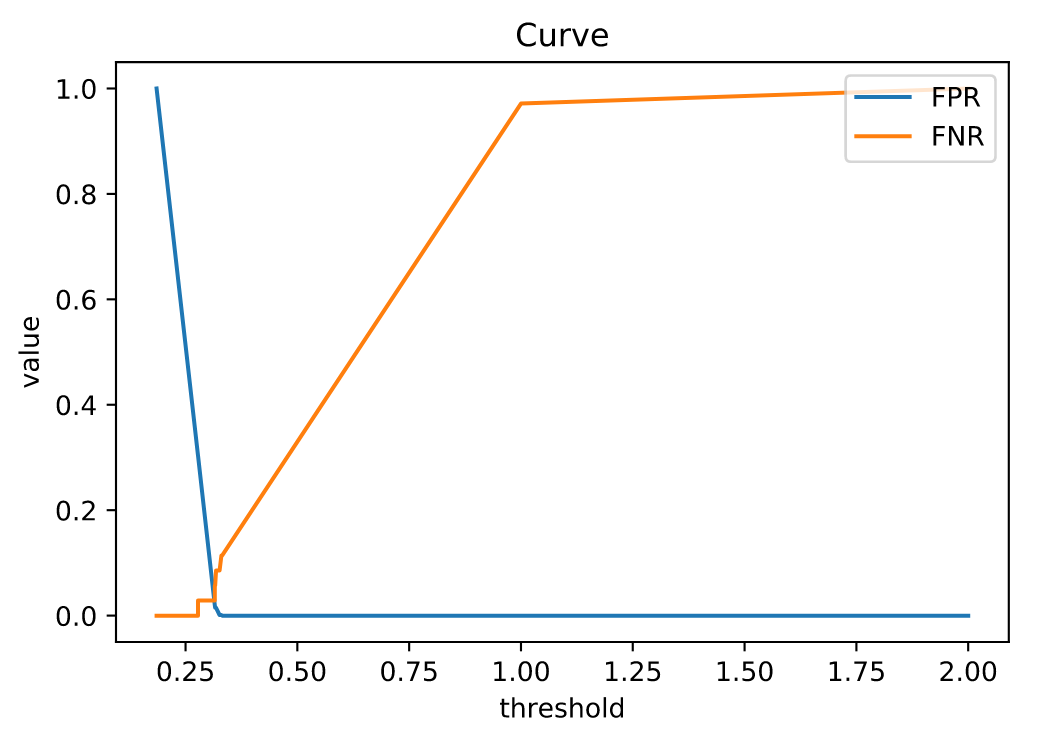
\includegraphics[scale=.35]{fpr_fnr_FDTW_Giovanni}
					\caption{FPR and FNR curve for the same user, EER is less than $ 0.01 $ and its relative threshold is approximately $ 0.03 $ }
				\end{center}
			\end{figure}
			
			\begin{figure}[H]
				\begin{center}
					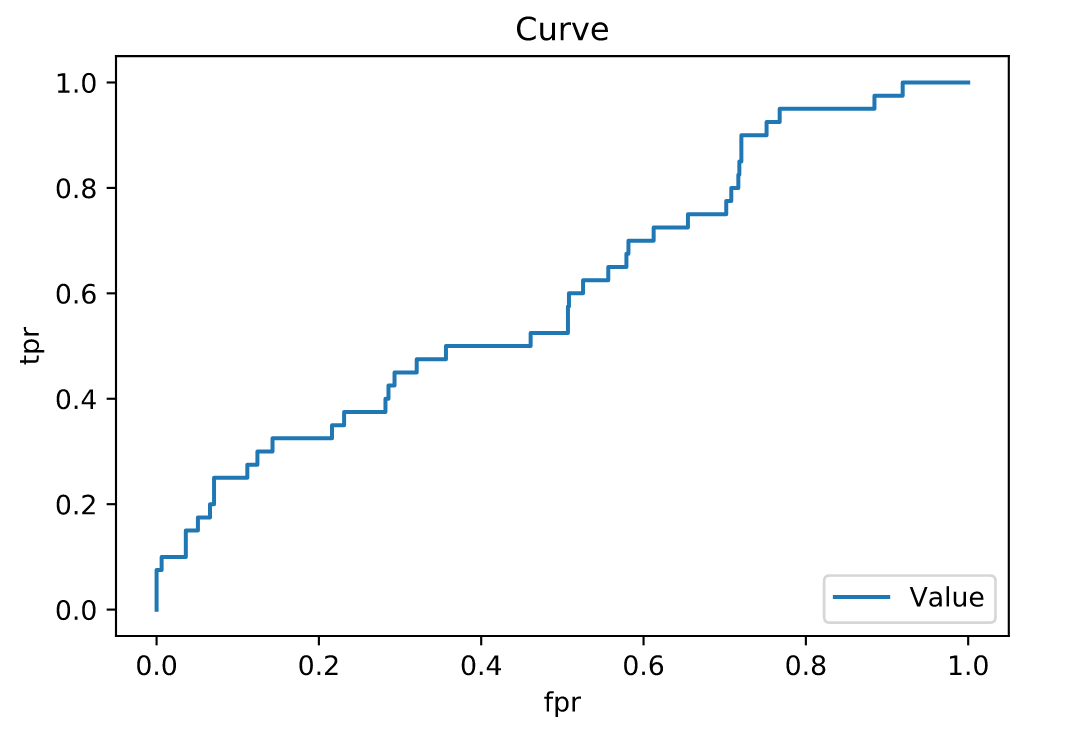
\includegraphics[scale=.35]{ROC_FDTW_Dario}
					\caption{ROC curve of one of the worst FDTW performances;\\ AUC $ \cong 0.60 $}
				\end{center}
			\end{figure}
			
			\begin{figure}[H]
				\begin{center}
					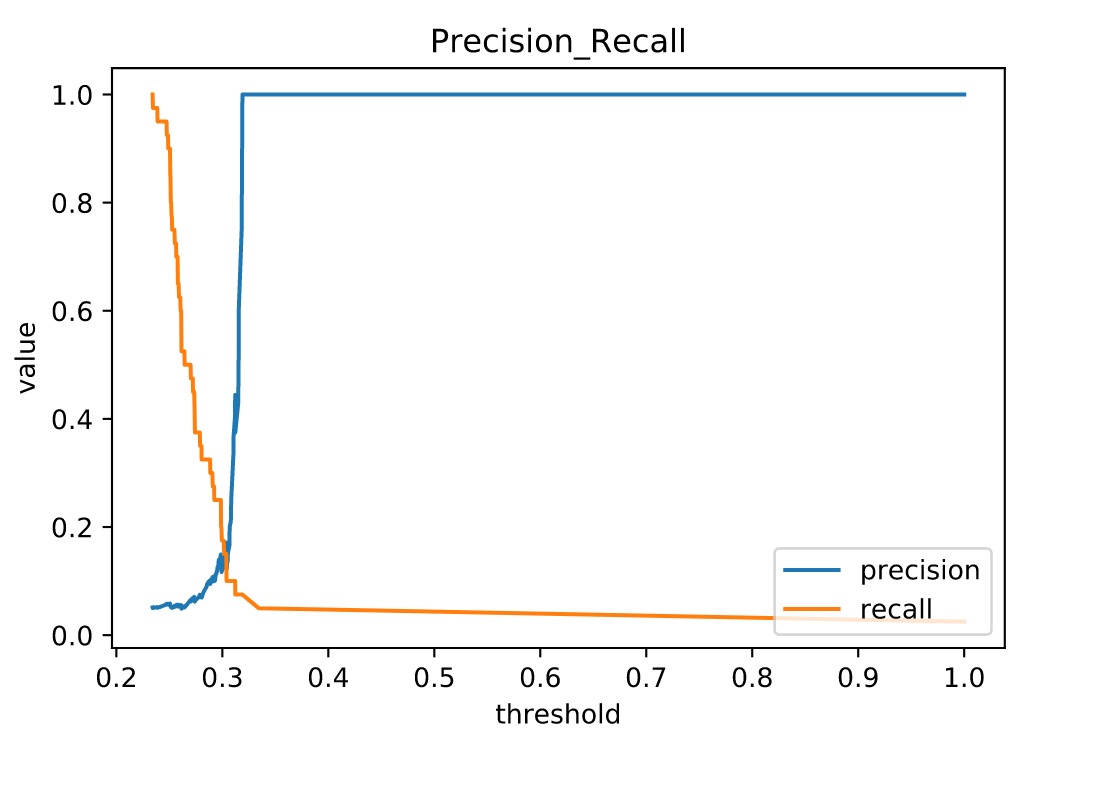
\includegraphics[scale=.35]{precision_recall_FDTW_Dario}
					\caption{Precision and recall curves for the same user}
				\end{center}
			\end{figure}
			
			\begin{figure}[H]
				\begin{center}
					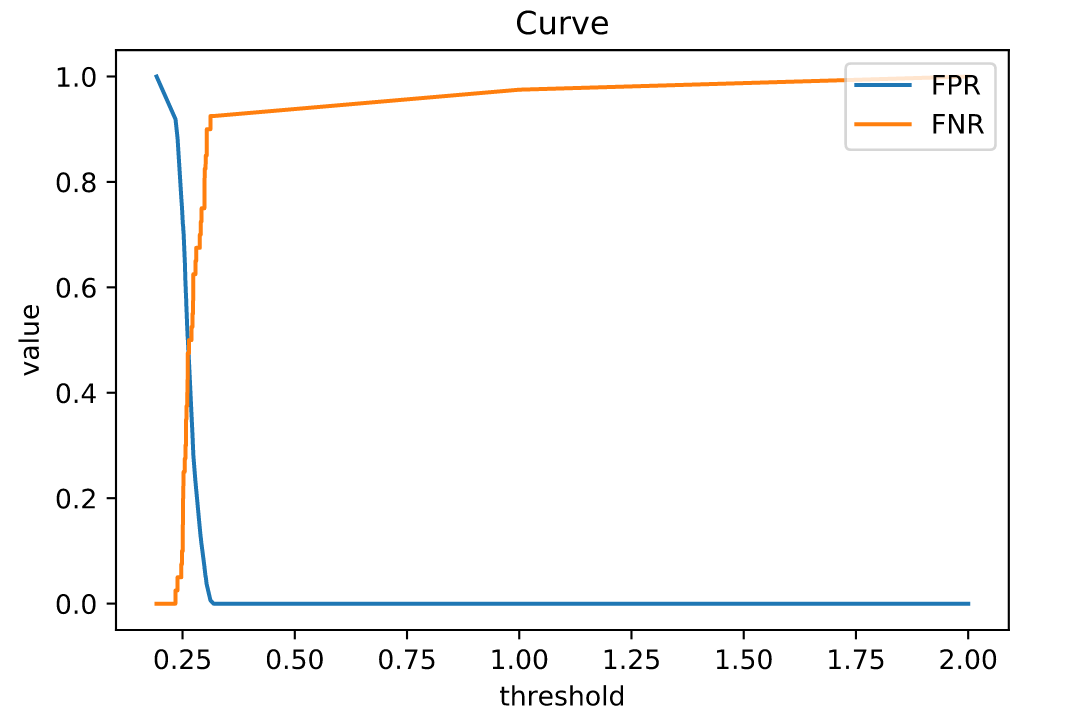
\includegraphics[scale=.35]{fpr_fnr_FDTW_Dario}
					\caption{FPR and FNR curve for the same user, EER is less than $ 0.5 $ and its relative threshold is approximately $ 0.3 $}
				\end{center}
			\end{figure}

		
		\subsection{LSTM}
		
			The LSTM model has reached very good performances in a rather small number of training epochs, always considering the limited dataset size. We present just two of the generated models and their relative tests, as other examples would be unnecessary. In both cases the model has obtained good results, reaching a precision of at least 98\%, both in the test and in the validation set; it should also be noted that we had more data for the first user, which could explain the better performance of the system when compared to the second user. 
			\begin{figure}[H]
				\begin{center}
					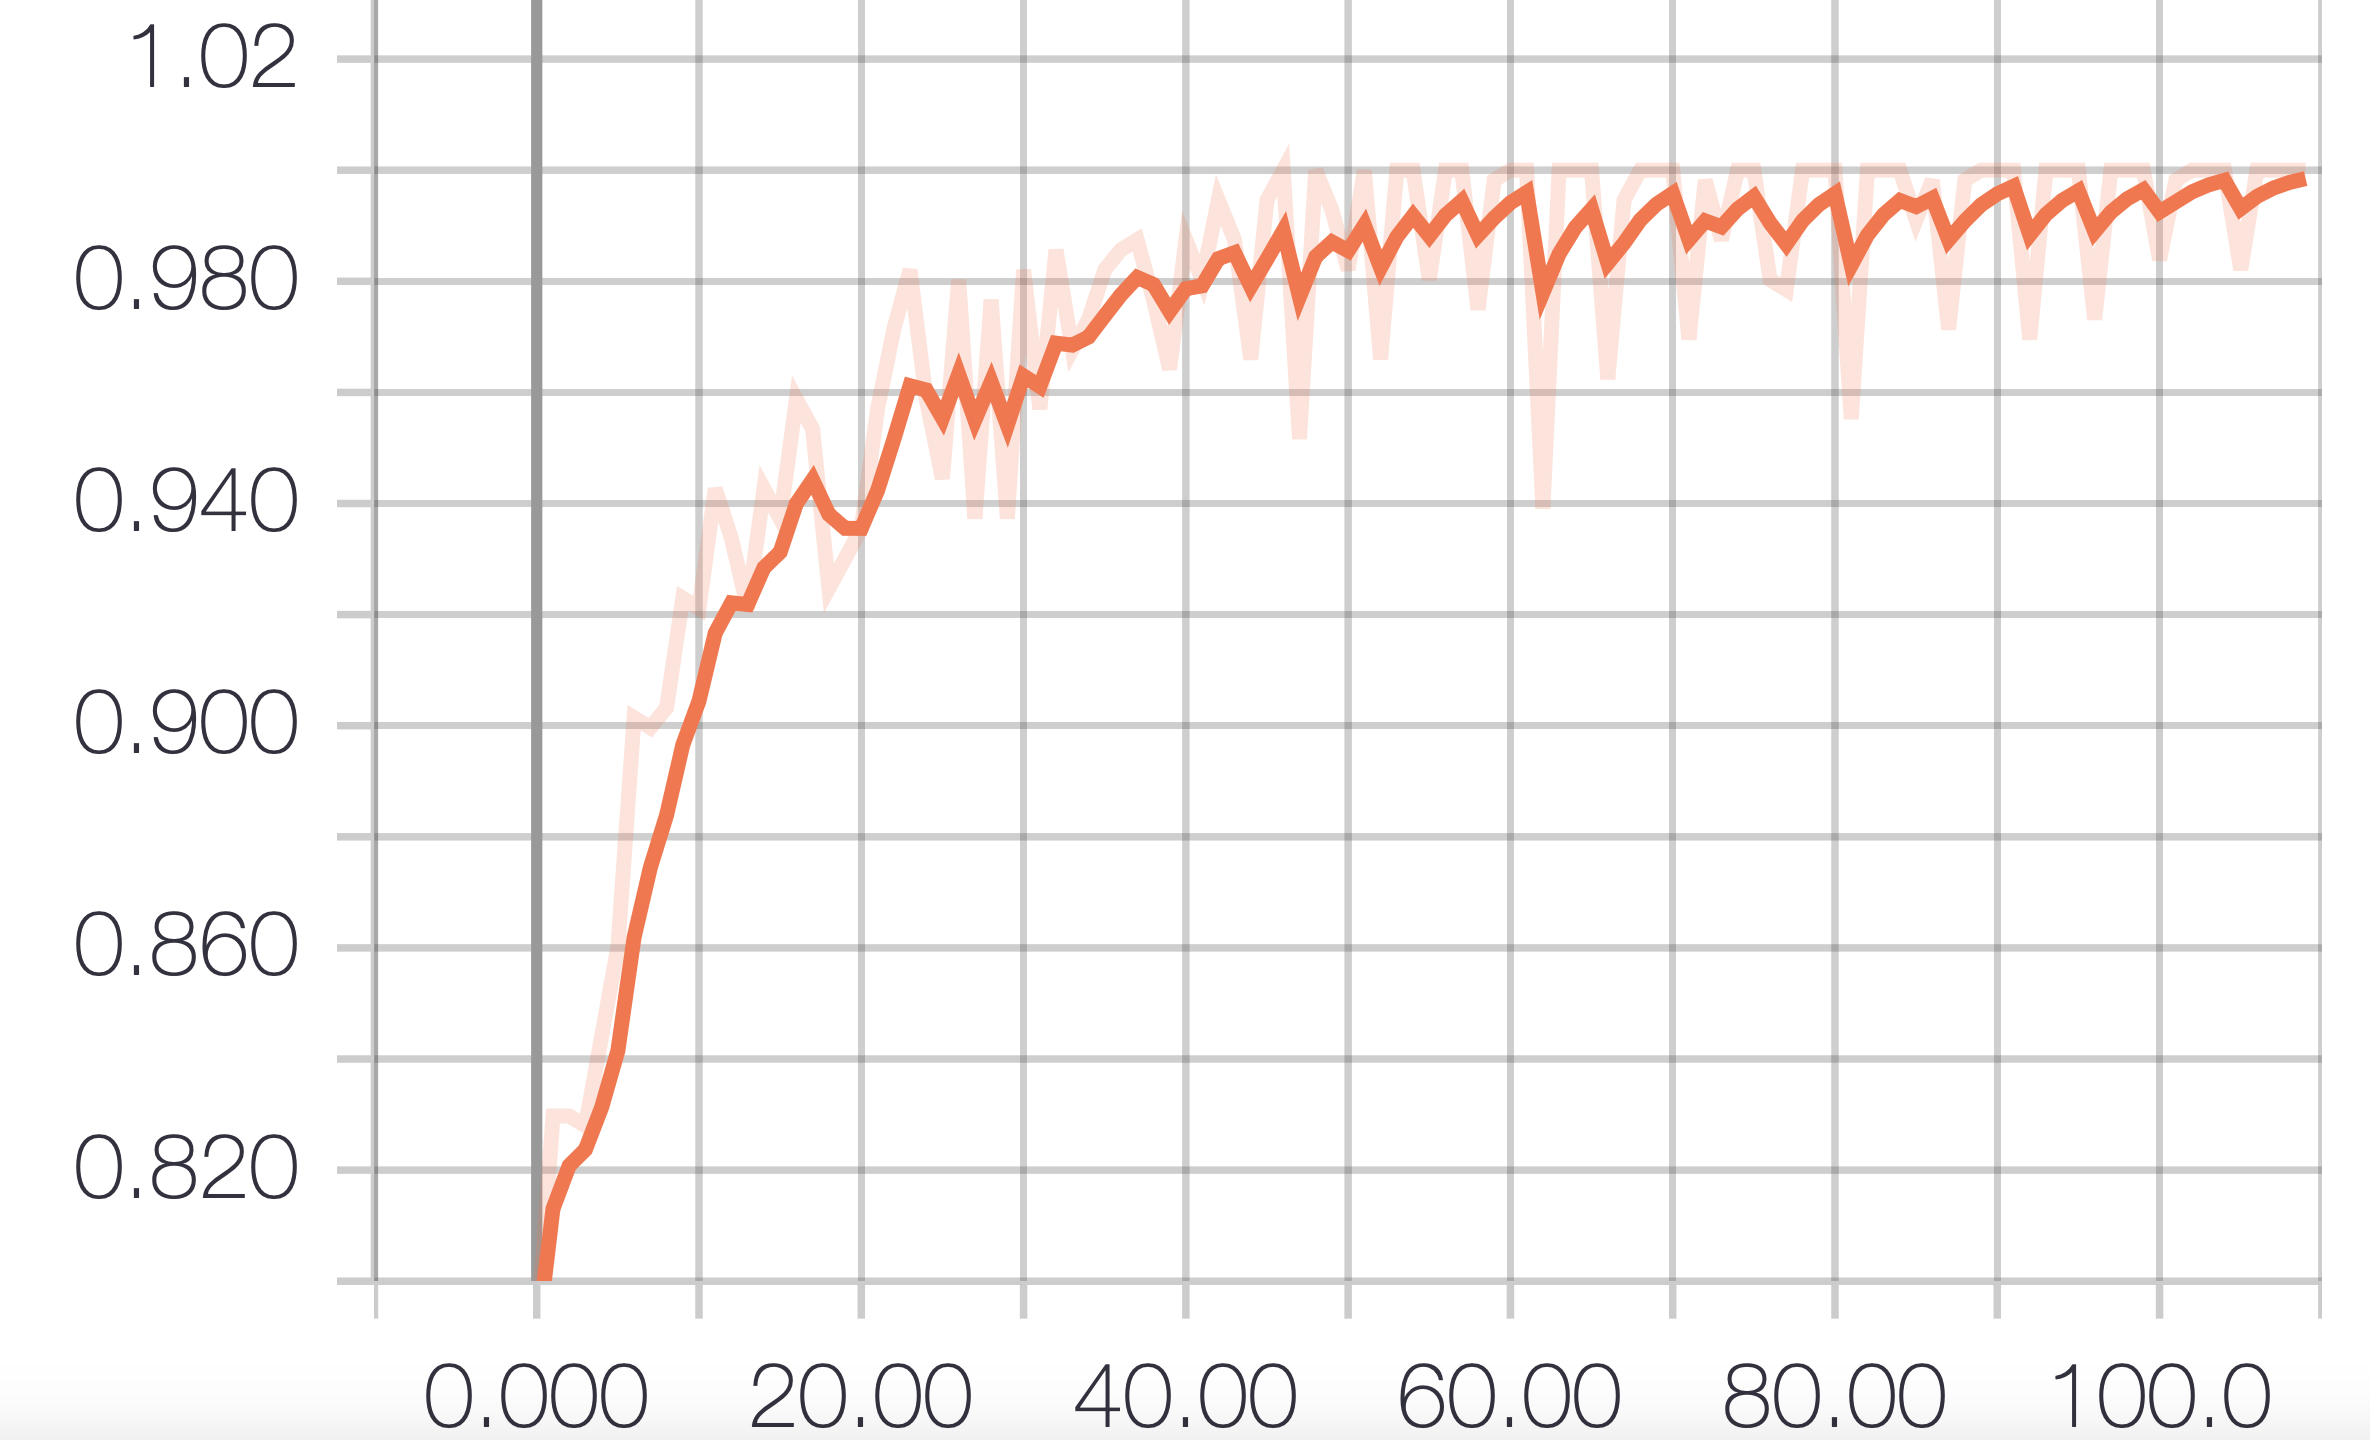
\includegraphics[scale=.1865]{acc_Antonio}
					\caption{Training set accuracy; first user}
					\label{fig:acc_train_Antonio}
				\end{center}
			\end{figure}
			
			\begin{figure}[H]
				\begin{center}
					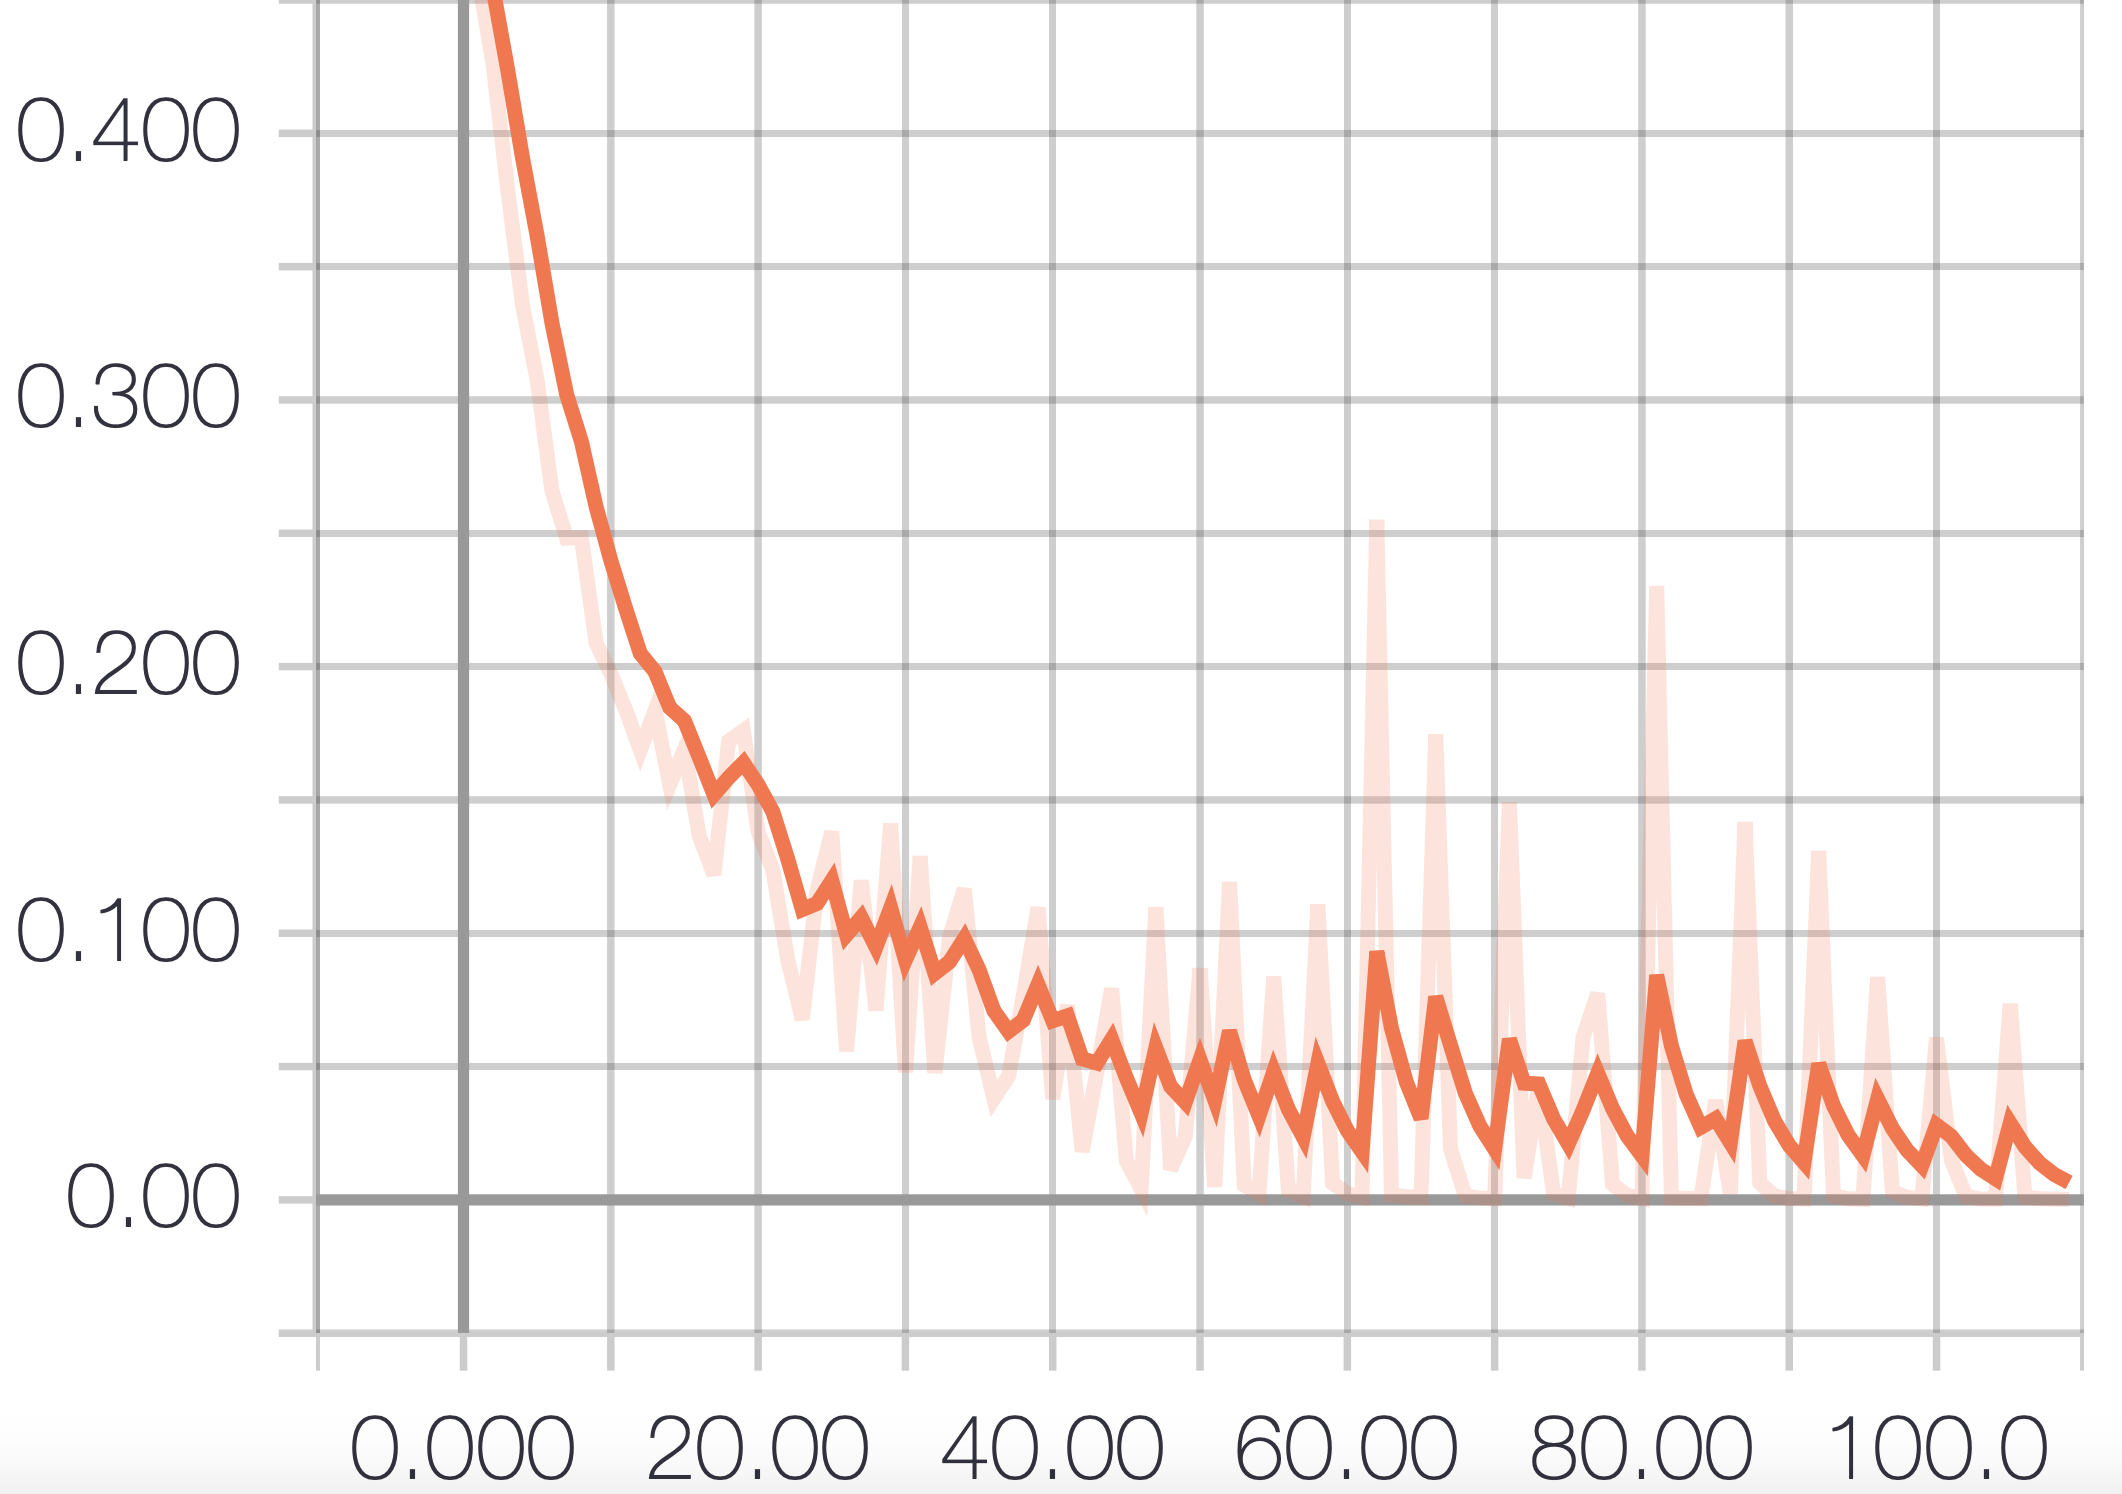
\includegraphics[scale=.1865]{loss_Antonio}
					\caption{Training set loss}
				\end{center}
			\end{figure}
			
			\begin{figure}[H]
				\begin{center}
					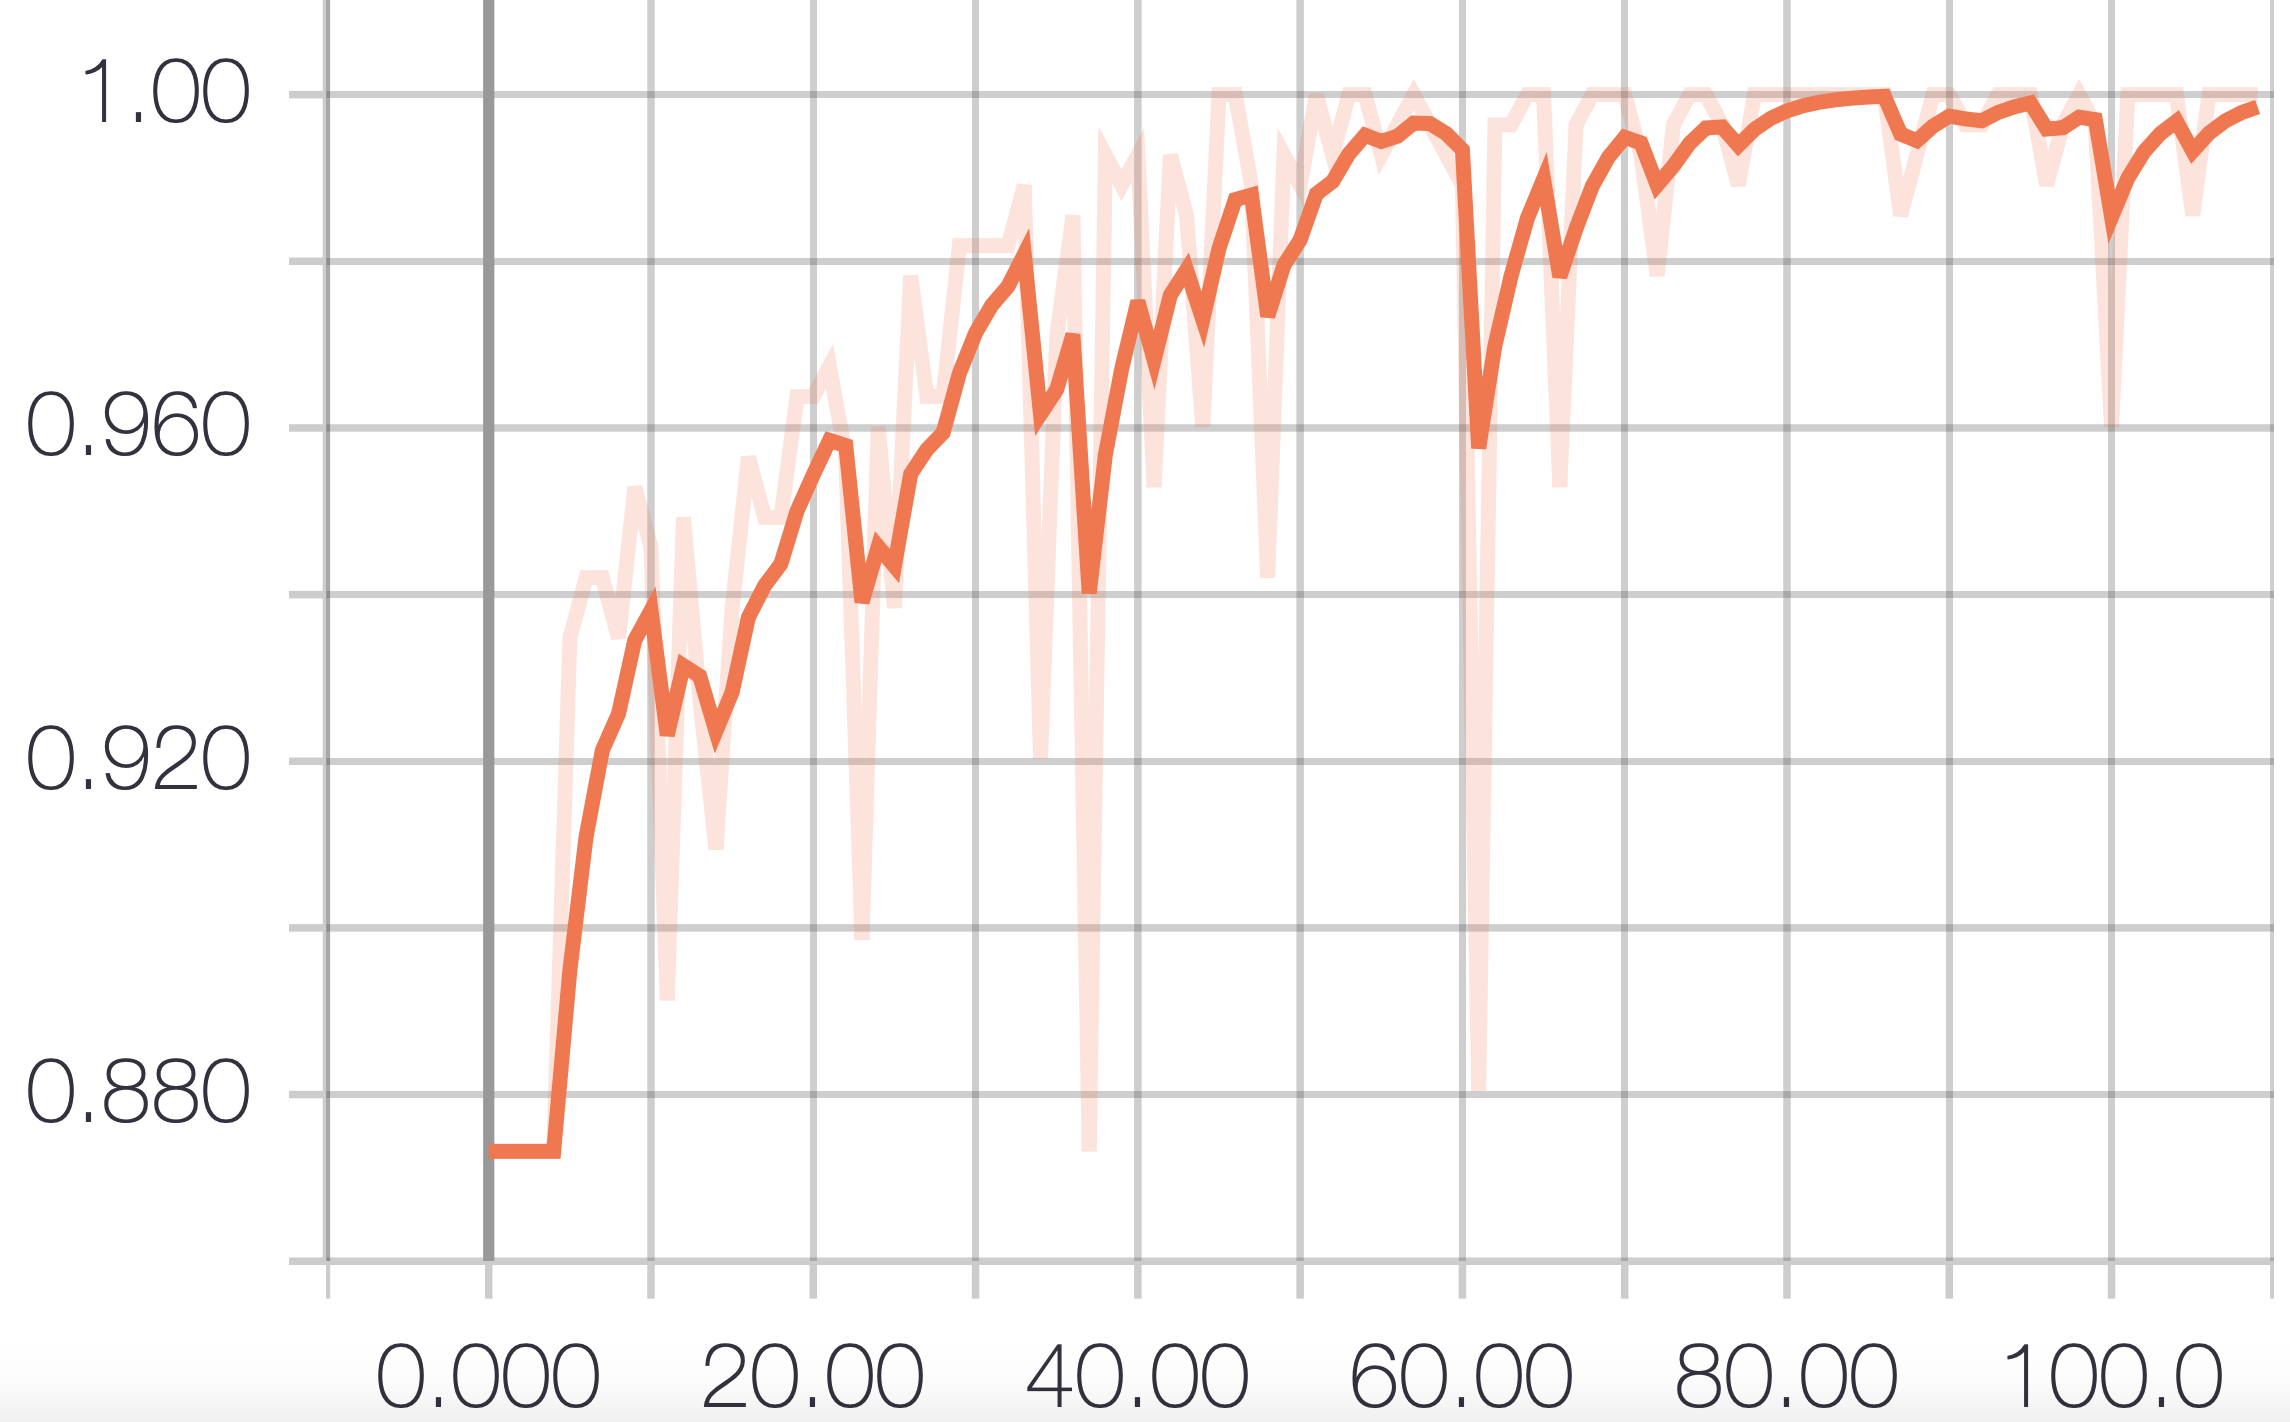
\includegraphics[scale=.1865]{val_acc_Antonio}
					\caption{Validation set accuracy}
					\label{fig:acc_val_Antonio}
				\end{center}
			\end{figure}
			
			\begin{figure}[H]
				\begin{center}
					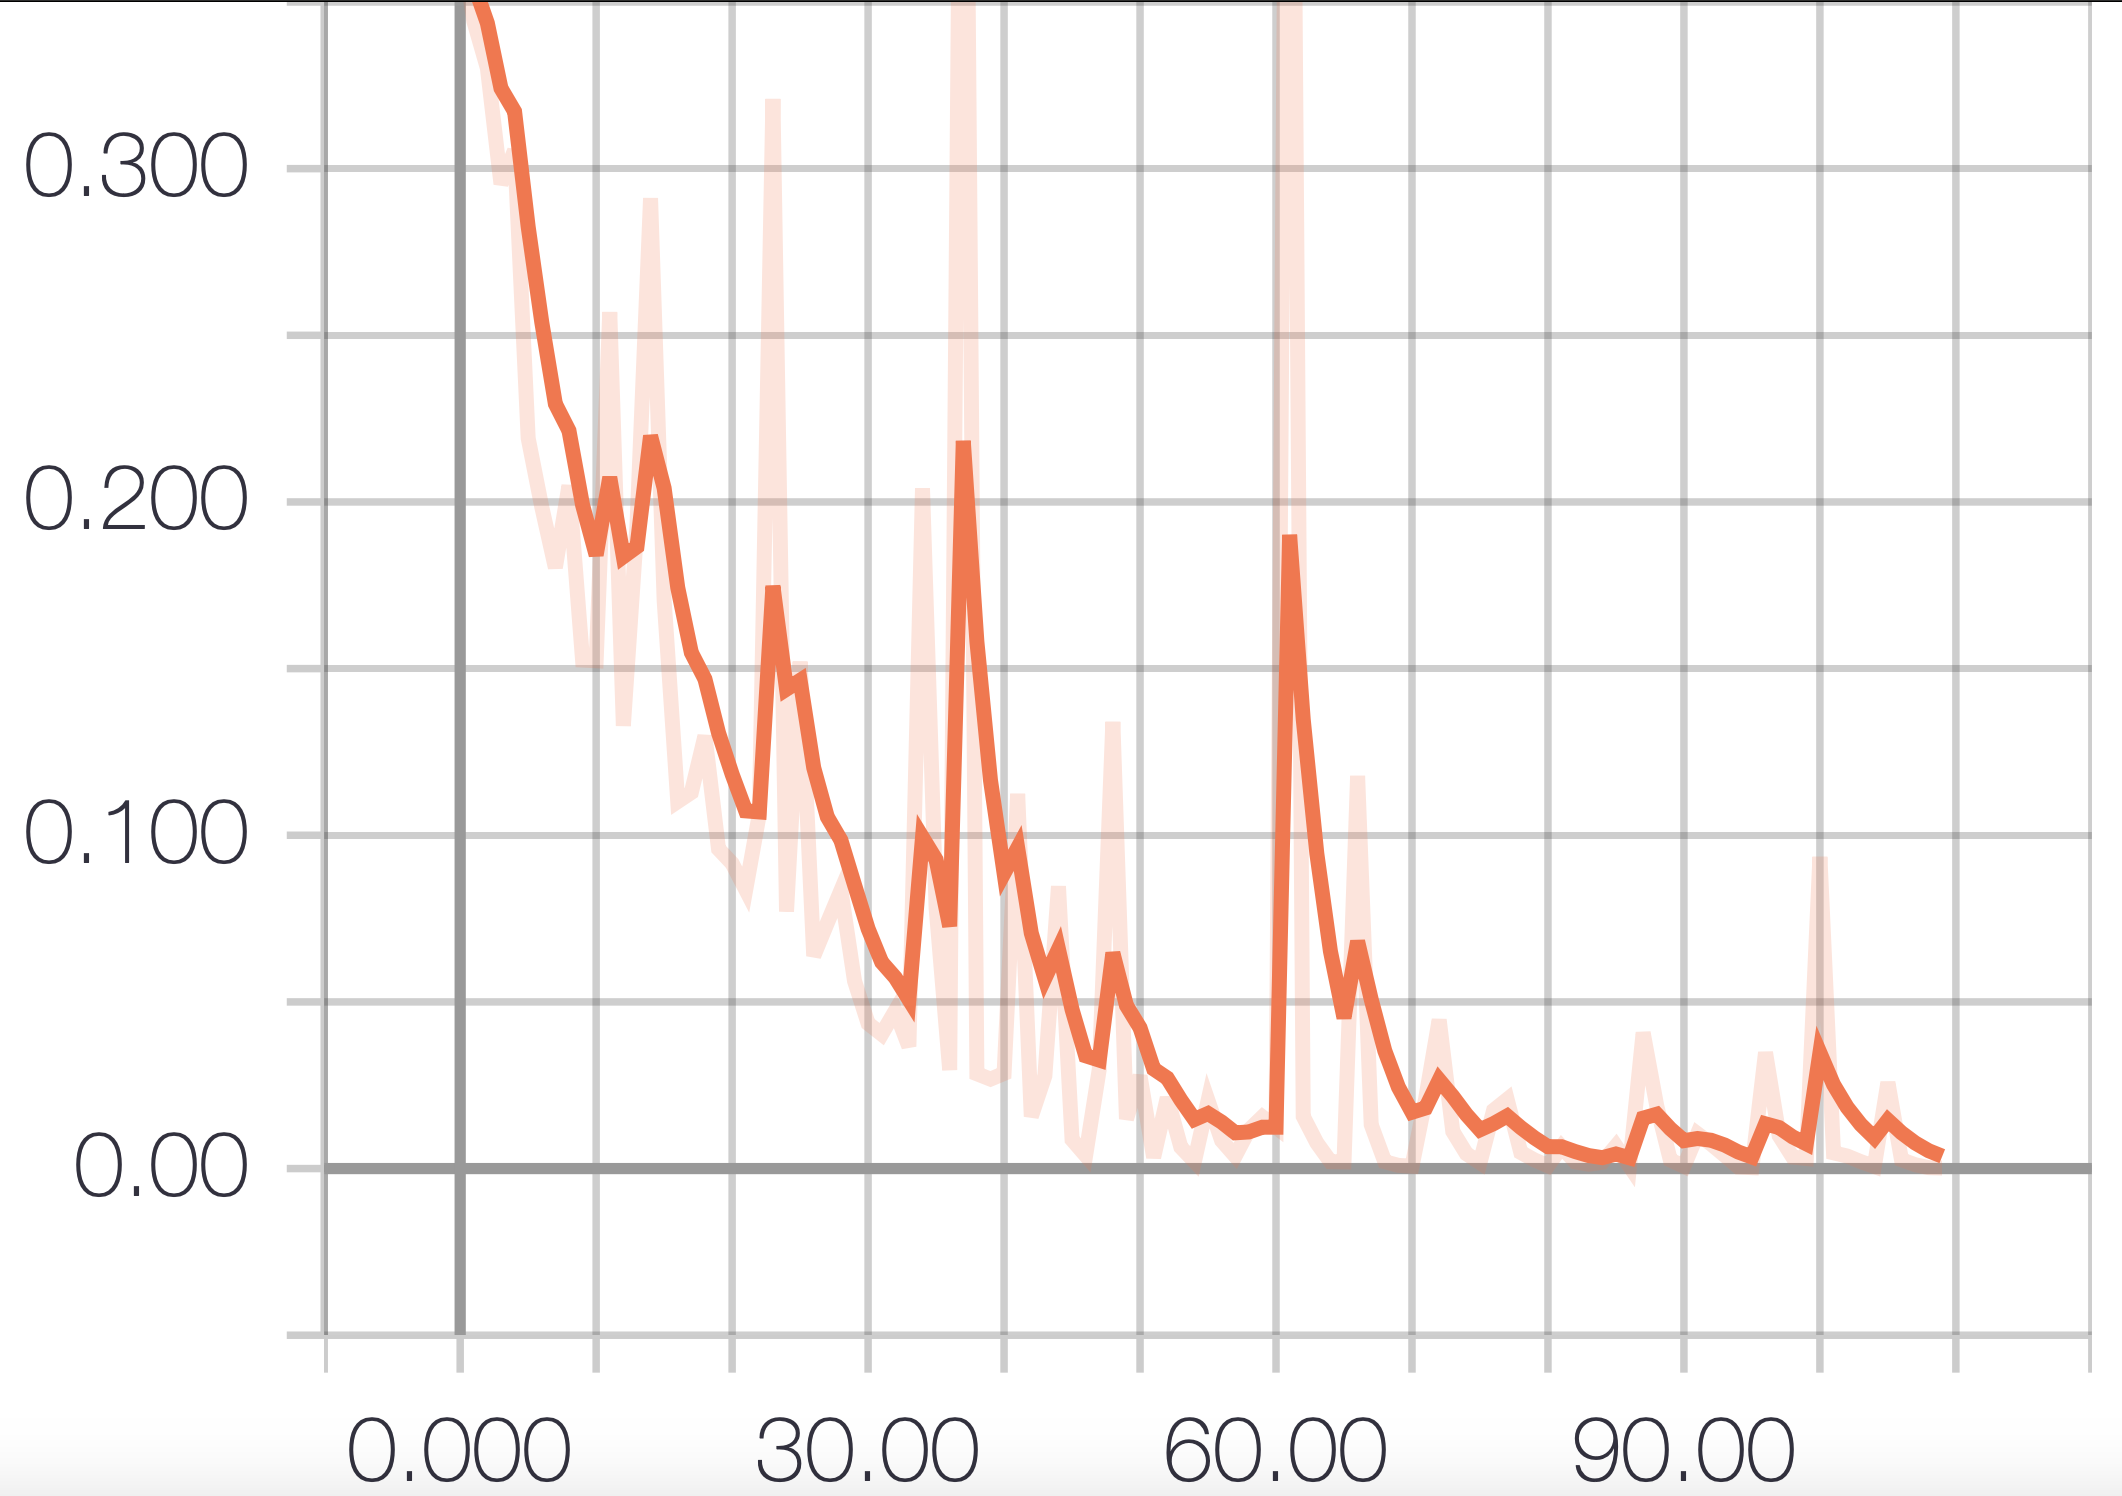
\includegraphics[scale=.1865]{val_loss_Antonio}
					\caption{Validation set loss}
				\end{center}
			\end{figure}
			
			\begin{figure*}
				\begin{center}
					\includegraphics[scale=.5]{test_Antonio}
					\caption{Classifications of the first model on some words written by its user in a different time}
					\label{fig:prediction}
				\end{center}
			\end{figure*}
			
			\newpage
			
			\begin{figure}[H]
				\begin{center}
					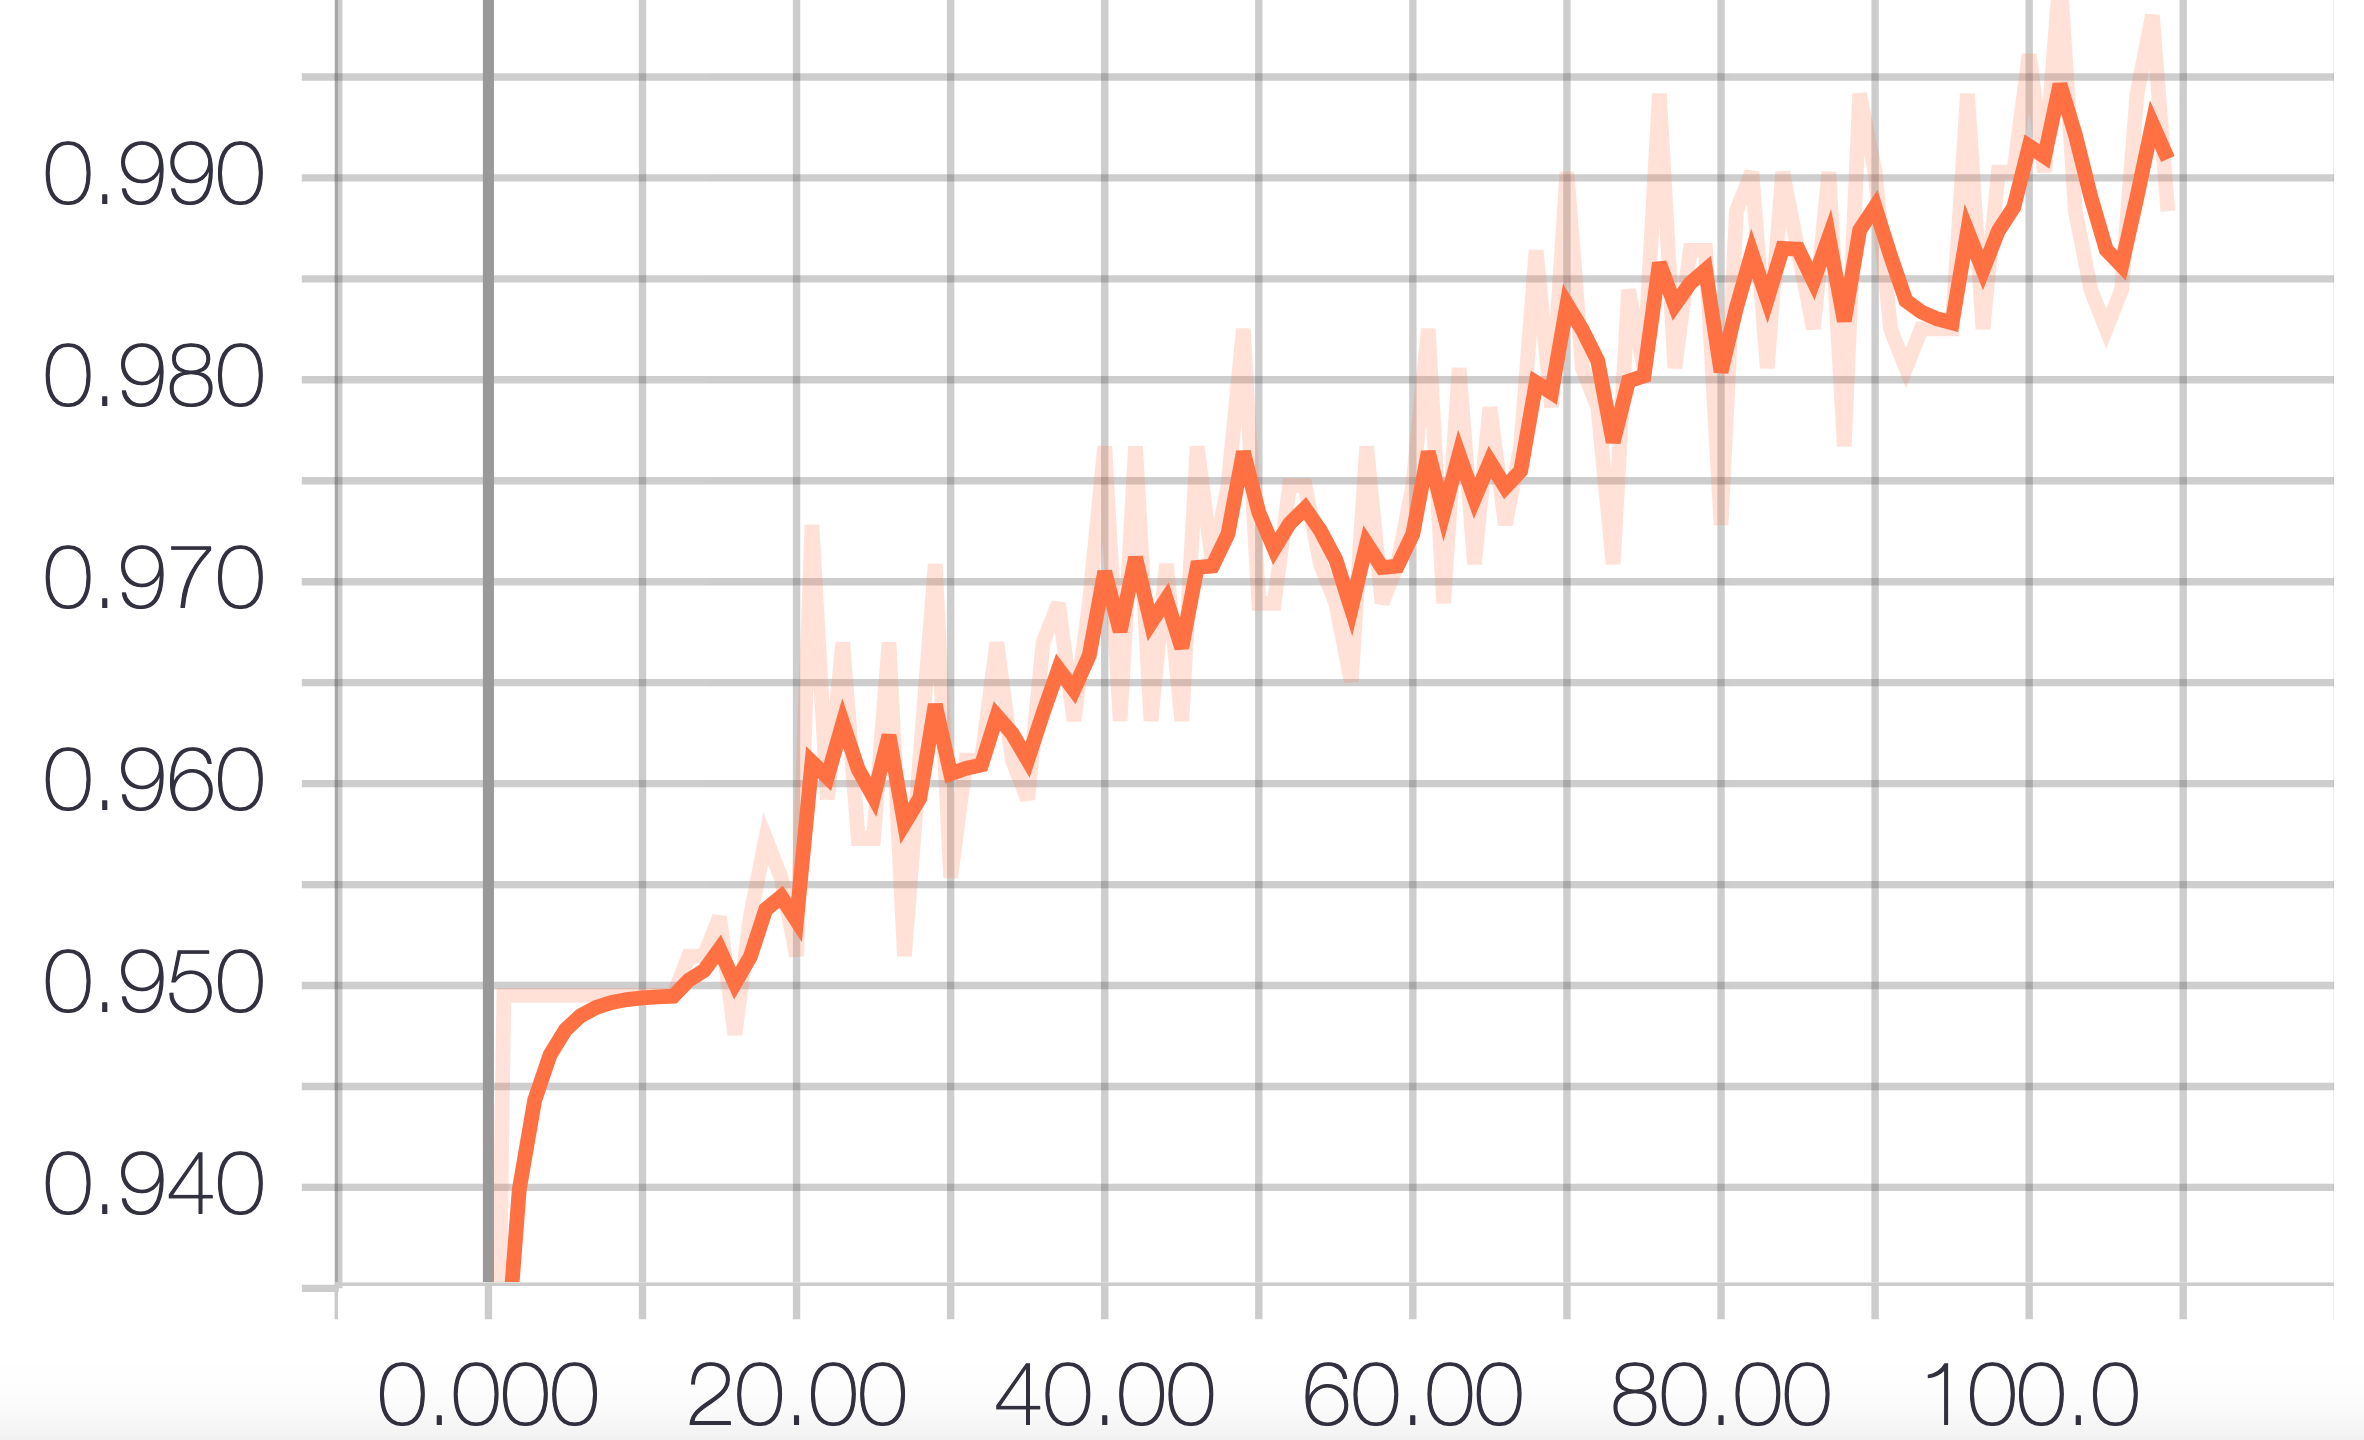
\includegraphics[scale=.16]{acc_Manuel}
					\caption{Training set accuracy; second user}
					\label{fig:acc_train_Manuel}
				\end{center}
			\end{figure}
			
			\begin{figure}[H]
				\begin{center}
					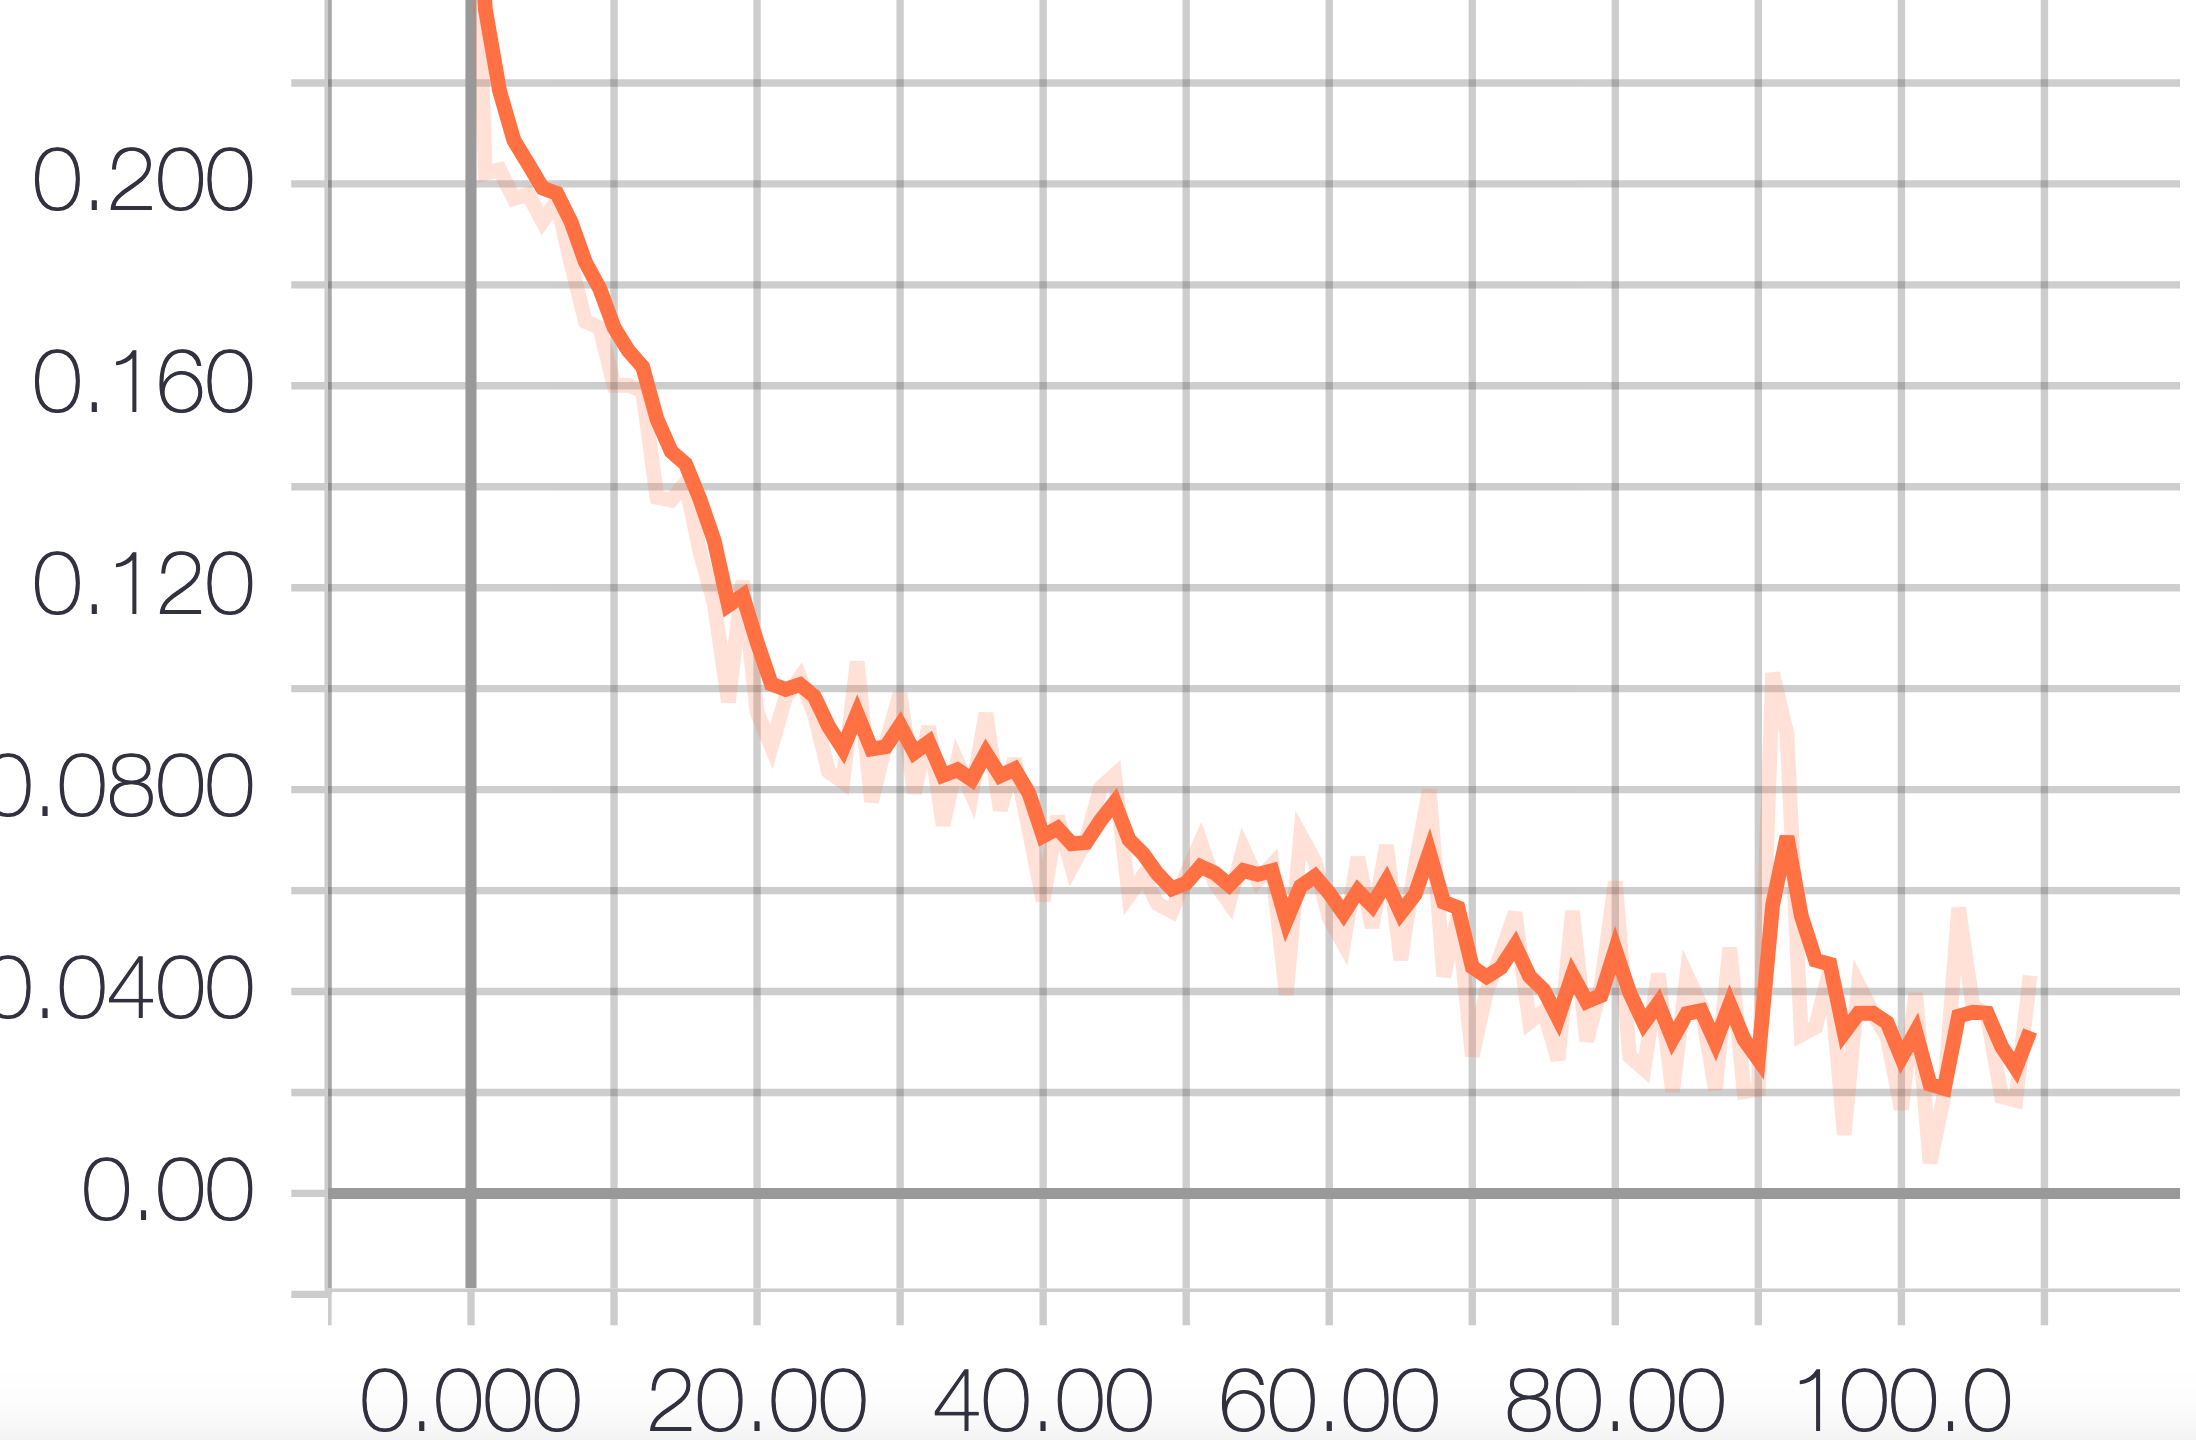
\includegraphics[scale=.16]{loss_Manuel}
					\caption{Training set loss}
				\end{center}
			\end{figure}
		
			\newpage
			
			\begin{figure}[H]
				\begin{center}
					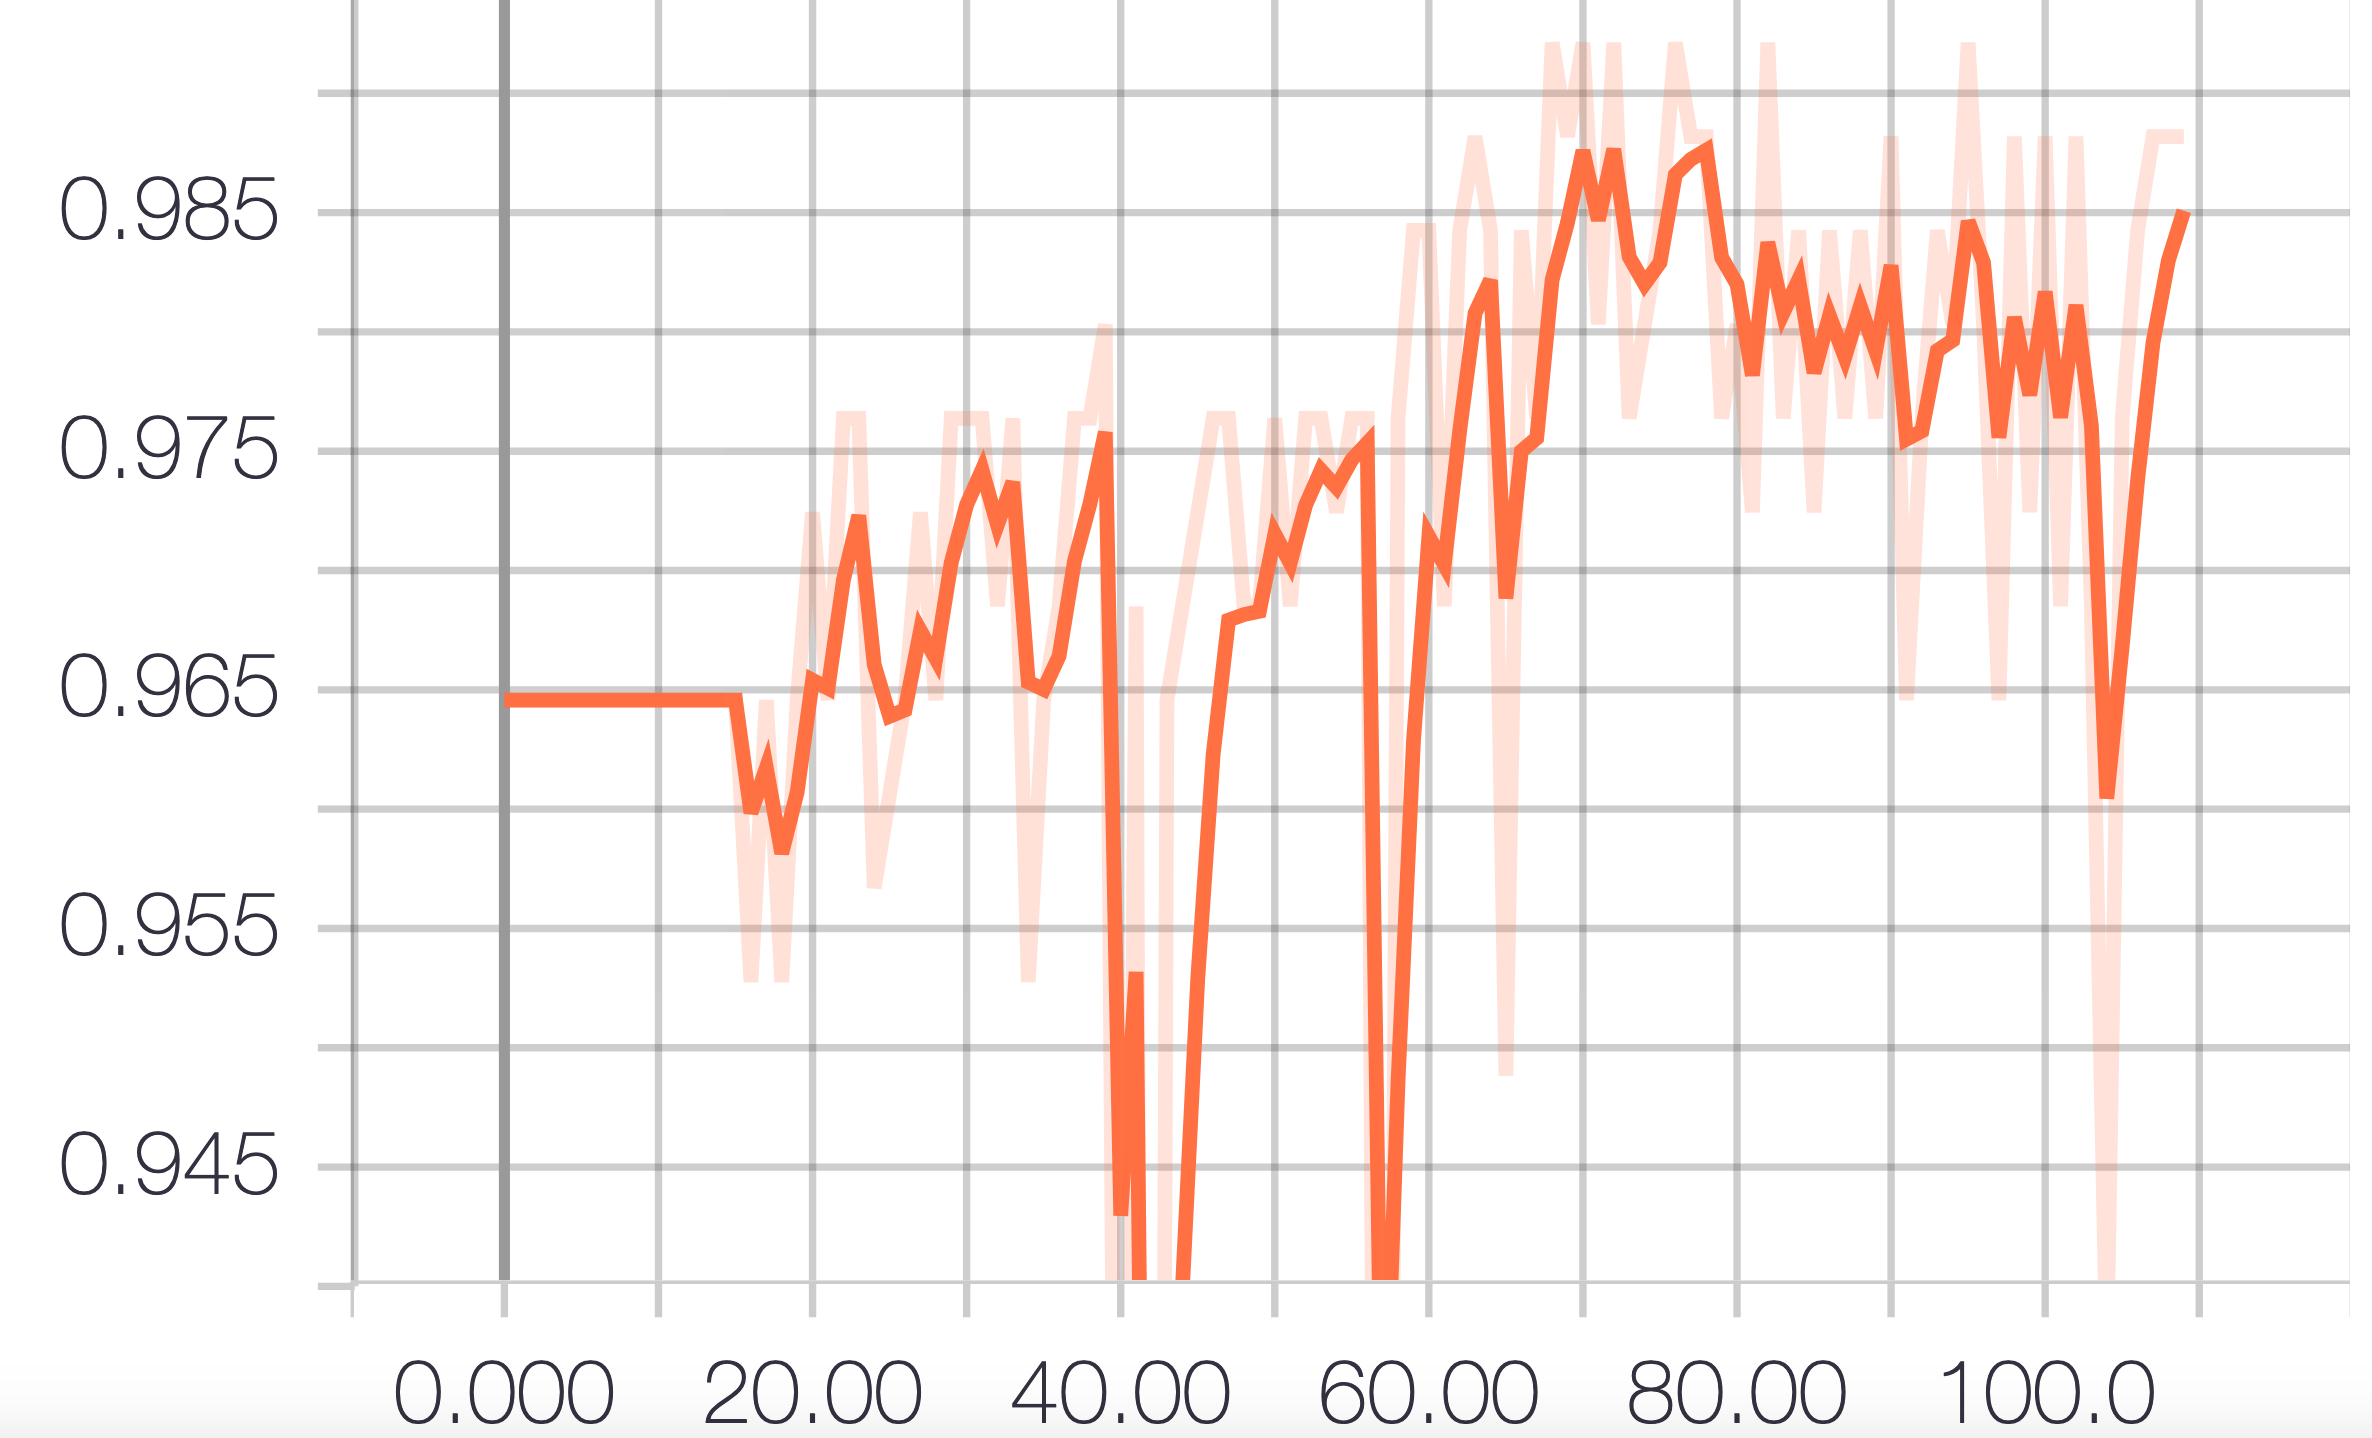
\includegraphics[scale=.16]{val_acc_Manuel}
					\caption{Validation set accuracy}
					\label{fig:acc_val_Manuel}
				\end{center}
			\end{figure}
			
			\begin{figure}[H]
				\begin{center}
					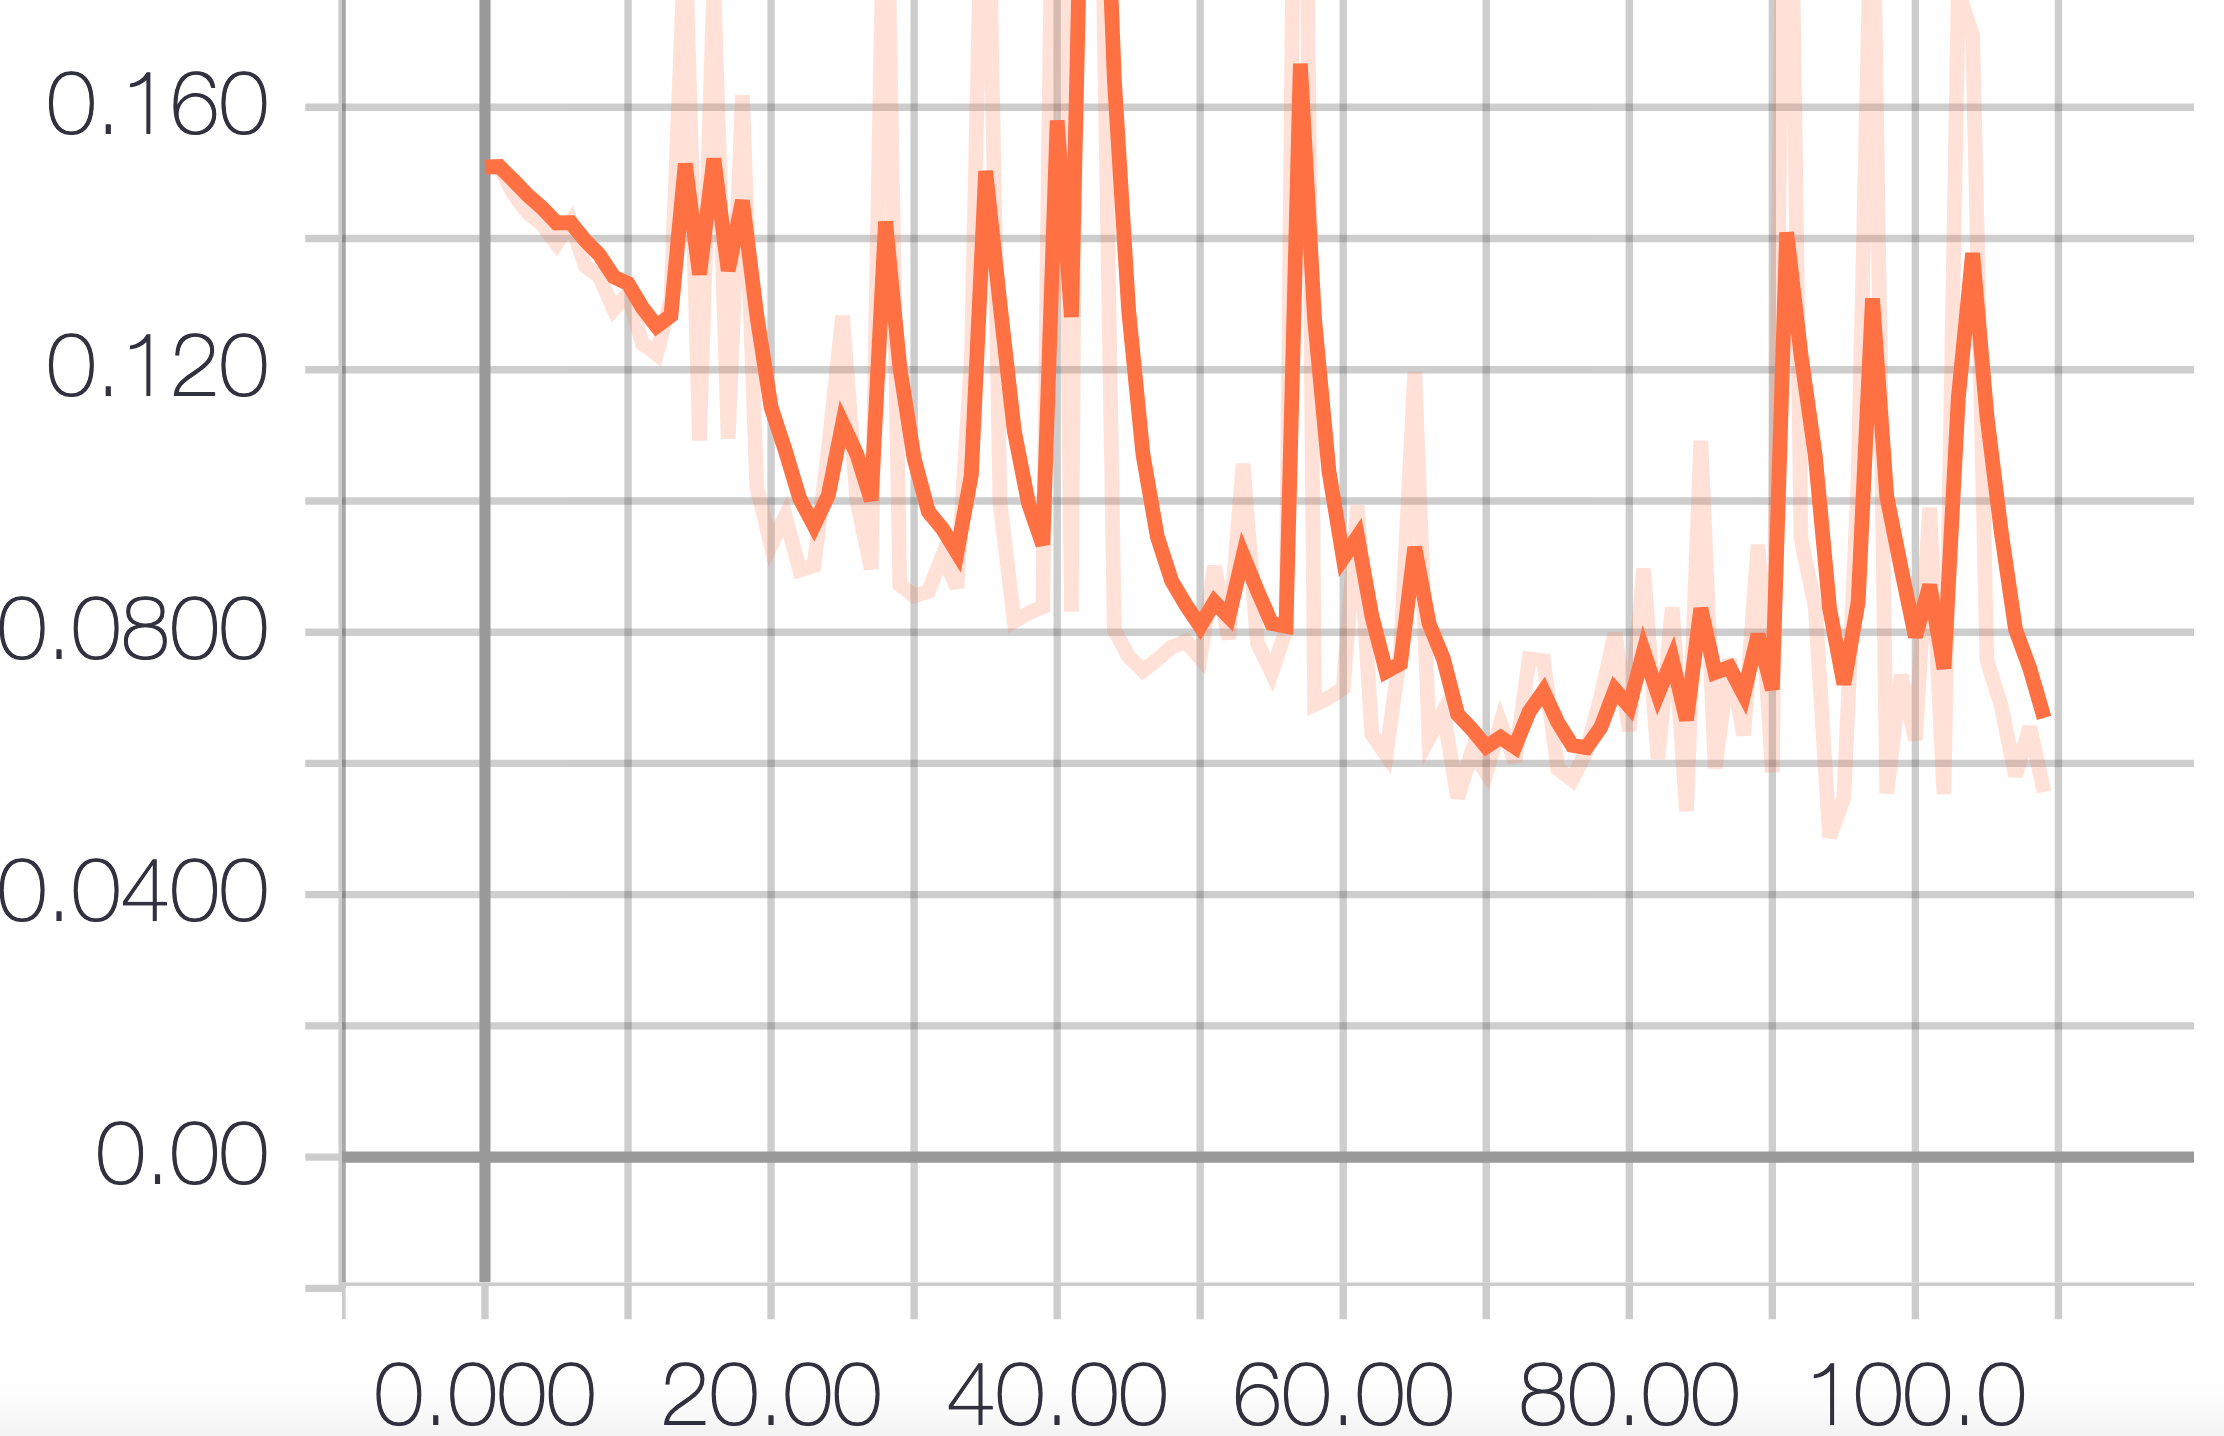
\includegraphics[scale=.16]{val_loss_Manuel}
					\caption{Validation set loss}
				\end{center}
			\end{figure}
			
			\newpage			
			
			\begin{figure}[H]
				\begin{center}
					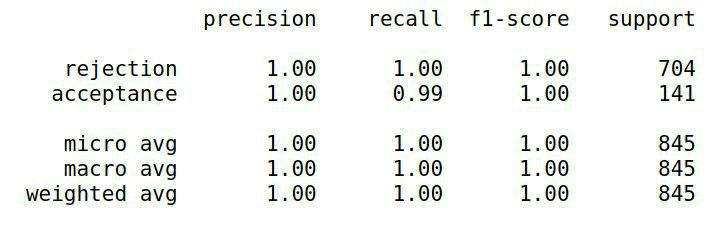
\includegraphics[scale=.4]{measures_table_LSTM}
					\caption{Statistics report for the first user model}
				\end{center}
			\end{figure}
			\newpage
			Especially interesting is the prediction figure, which represents the PeterPen's main task, i,.e. recognize a user from data obtained while writing, using a model trained on the same user's data but obtained in a previous time. From the performed tests it seems that the model achieves this goal, with a precision of almost 99\% (\cref{fig:prediction}). \\
			Moreover, there seems to be no overfitting or underfitting, as it reaches very similar accuracies in the last epochs for the training set (\cref{fig:acc_train_Antonio}, \cref{fig:acc_train_Manuel}) and the validation set (\cref{fig:acc_val_Antonio}, \cref{fig:acc_val_Manuel}).


\chapter{Future works}

	Firstly, we would like to print a better case. Putting together the pen has proved to be a quite difficulta task, mainly due to the printer's low precision. \\
	Secondly, a dedicated chip would be ideal, as the majority of the available pins on the ESP8266 have not been utilized. \\
	Concerning software, there could be two possible developments. \\
	For DTW, we could try to weigh the single features in evaluating the costs. This idea has risen from the observation that, with a high chance, when evaluating the distance between two written words, some data components could be more important than others. Also, more tests must be performed, in order to further verify the system's performances with a higher precision. \\
	Finally, we have observed that the deep learning model, which was trained only on the word "Computer" written by a user, has "incorrectly" recognized some "Ciao"s written by the same user (\cref{fig:ciao}). This could prove that, with high chances, the system could effectively be used to recognize a user by his or her handwriting, provided that the model is trained on various words written by the same one.  
	
	\begin{figure}[H]
		\begin{center}
			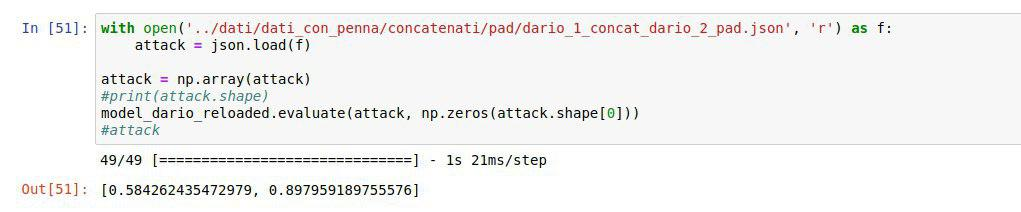
\includegraphics[scale=.3]{scrittura_dario}
			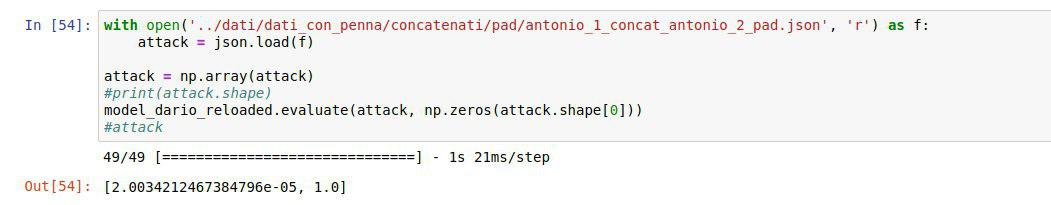
\includegraphics[scale=.3]{scrittura_antonio}
			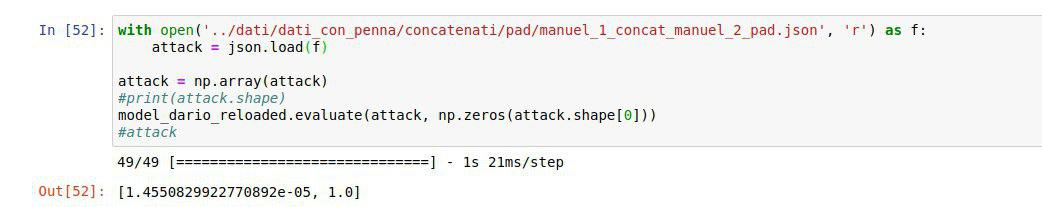
\includegraphics[scale=.3]{scrittura_manuel}
			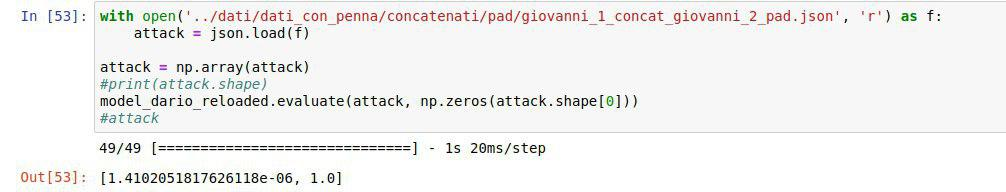
\includegraphics[scale=.3]{scrittura_giovanni}
			\caption{As it can be seen, the model rejects (correctly) the impostors, while in about 10\% of the cases it correctly recognizes the user, even though it has never seen that word}
			\label{fig:ciao}
		\end{center}
	\end{figure}



\bibliographystyle{myIEEEtranS}
\bibliography{mybib}{}

\end{document}